\documentclass[]{UCD_CS_FYP_Report}
\usepackage{graphicx}
\usepackage{hyperref}
\usepackage{subcaption}
\usepackage{amsmath}
%%%%%%%%%%%%%%%%%%%%%%
%%% Input project details

\def\studentname{Yue Xiao} % Edit with your name
\def\projecttitle{Deep Learning - Image segmentation} % Edit with you project title
\def\supervisorname{Neil Hurley}

\begin{document}

\maketitle

%%%%%%%%%%%%%%%%%%%%%%
%%% Your Project Specification

\chapter*{Project Specification}
Image segmentation is an important field in computer vision. It consists on dividing the image to extract the regions of interest by assigning a label to every pixel such that pixels in a region will have the same pixel. Historically, computer vision has used image processing techniques for segmentation and machine learning for labelling; but deep learning became popular with ImageNet 2012.

The first experiment in image segmentation with deep learning involved a sliding window setup where a patch around the pixel is taken which provides local context. A benefit of this approach was that training data is significantly larger than pixels available, which helps for applications such as medical image segmentation where training data is low. On the other hand the disadvantages are that the optimal patch size is hard to be obtained and it has to be applied on all pixels; and there is a lot of redundancy in the available data. Increasing the patch size gives more contextual information but they require more number of max pooling layers, and consequently lower localization accuracy. These problems were solved with fully convolutional networks like FCN and UNet. These networks has been a milestone in the history of image segmentations such as Alexnet in classification.

It is important to note that deep learning still requires a significant amount of labelled data, which is not available in many domains.

The main ideas behind networks such as FCN and UNet are:
\begin{enumerate}
\item {The later layers have features which help explain what the image contains. However, for exact localization of objects of interest we need more high-resolution features. Therefore, skip connections are used to combine information from the earlier layers with the low resolution information from the deeper layers.} 
\item {Using deconvolution networks for up-sampling.}
\item {UNet also introduced a different cost function which gives higher weightage to error in borders. This leads to models with more precise segmentations.}
\end{enumerate}
Core: 
The project will involve the following mandatory tasks:
\begin{enumerate}
\item {Choose a public dataset and define the problem. Prove understanding of the problem.}
\item {Apply a deep network for image segmentation in the problem chosen.}
\end{enumerate}
Advanced: 
Advanced (choose one or both):
Develop an example applying semantic segmentation.
Apply transfer learning to apply the trained network in a different application ( a different dataset).

%%%%%%%%%%%%%%%%%%%%%%
%%% Your Abstract here

\begin{abstract}

\textbf{\textsl{Image classification is a very important field in computer vision. Recent years, deep learning has become a very popular method in this field and the Deep Neural Networks, which are trained on large datasets, are currently one of the most popular approaches for image classification. To develop deep neural networks for image classification, this project consists of three main parts: the background research on the principle of artificial neural network, and solve two problem, the classification of MNIST dataset and the classification of CIFAR-10 dataset, using deep neural network.}}

\textbf{\textsl{In background research, the basic principles of Neural Network and its training process are discussed. Then, for the classification of MNIST database, two models, one fully-connected neural network and one convolutional neural network, are developed and trained, and achieves an accuracy of 98.35\% and 99.17\% respectively. For the classification of CIFAR-10 database, a benchmark is chosen from the state-of-the-art approaches on this problem. After that, a convolutional neural network model is developed and trained, and achieves an accuracy of 84.64\%. The details about the development of these deep neural network models will be covered in this report.}}
\end{abstract}
\newpage


%%%%%%%%%%%%%%%%%%%%%%
%%% Acknowledgments

\chapter*{Acknowledgments}

I would like to express my very great appreciation to Dr. Raul Moreno Salinas and Dr. Armita Afsharinejad for their patient guidance and precious suggestions during the planning and development of this project.

I would also like to thank Prof. Neil Hurley, my supervisor, for his professional guidance and valuable support.

%%%%%%%%%%%%%%%%%%%%%%
%%% Table of Content

\tableofcontents\pdfbookmark[0]{Table of Contents}{toc}\newpage
\newpage


%%%%%%%%%%%%%%%%%%%%%%
%%% Introduction

\chapter{Introduction}
Image classification is a difficult task for computer, especially for the images contain complicated objects. With the popularity of deep learning in machine learning field in recent years, deep neural network now is one of the most popular approaches to perform this task. However, the theories of this technology is quite complicated, and the development and training process of Neural Network are intricate too. 

The object of this project is to understand the principle of neural network and practiced the theory in solving two problems, the classification of MNIST dataset and CIFAR-10 dataset. Therefore, this project consists of three main parts, the background research, and the development of deep neural networks for classifying MNIST and CIFAR-10 dataset. This report will cover these parts in three separated chapters.

In Chapter~\ref{chapter2}, this report will discuss the principle of artificial neural network and some important conceptions in its training process. Then, about the classification of MNIST dataset, since there were two different kinds of neural network models were used to solve this problem, the fully-connected neural network model and the convolutional neural network, this report will cover the development and training process of these two models respectively in Chapter~\ref{chapter3}. After that, to solve the second problem, the classification of CIFAR-10 colour images, a benchmark is chosen from the state-of-the-art approaches and a convolutional neural network is developed to improve the state of the art. The convolutional neural network for this problem is based on the best model build for MNIST database. The details of the benchmark and the process of building this convolutional neural network model will be discussed in Chapter~\ref{chapter4}. The implementation of neural network model and evaluation are covered in Chapter~\ref{chapter5}. In last Chapter, this report will discuss the conclusions and the future work.

The topic of this project is slightly different to the project specification, because my supervisor decided to change the topic from Image Segmentation to Image Classification. 

%%%%%%%%%%%%%%%%%%%%%%
%%% Background Research

\chapter{\label{chapter2}Background Research}
The principle of neural network is vital for this project. In this chapter, the conception of the artificial neural network will be discussed first. After that, this chapter will introduce three important types of neural networks and the training of feedforward neural network.
\section{Basic Conception of Artificial Neural Network}
Neural Network, also called Artificial Neural Network, is a kind of connectionist deep learning model inspired by the biological neural network, which consists of a series of interconnected neurons. Neural Networks contain many simple units, called artificial neurons, which are working in parallel. The weight between the units are the primary means of long–term information storage in neural network~\cite{Gibson:2017}. By updating the weights, neural network can learns new information from training. Neural Network can perform some complex tasks, such as solving complex signal processing, machine translation and pattern recognition problems, by learning existing examples.

The architecture of neural network can be defined by:
\begin{enumerate}
\item Number of neurons
\item Number of layers
\item Types of connections between layers~\cite{Gibson:2017} 
\end{enumerate}
%%%%%%%%%%%%%%%
\subsection{Artificial Neuron}
An artificial neuron is a mathematical function conceived as a model for a real biological neuron~\cite{Bonnin:2016}. The artificial neuron takes one or more inputs and feed them in to a transfer function, for example calculating the dot product of weights and inputs. Then pass through the result to an activation function to get an activation value. The Figure~\ref{fig:The architecture of Artificial Neuron} shows the architecture of an artificial neuron.
\begin{figure}[h]
\centering
\fboxsep 2mm
\framebox{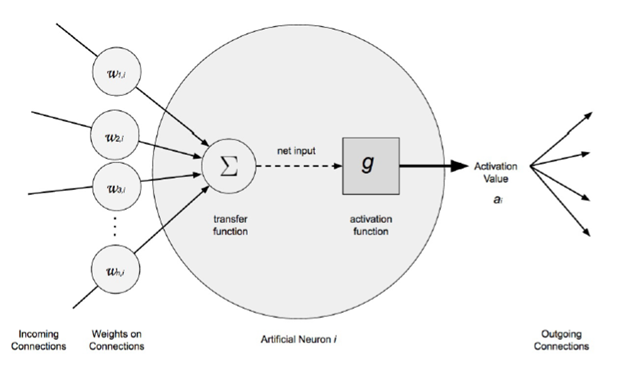
\includegraphics[width=6cm]{Images/The_architecture_of_Artificial_Neuron.png}}
\caption{\label{fig:The architecture of Artificial Neuron} The architecture of Artificial Neuron~\cite{Gibson:2017}.}
\end{figure} 
\subsection{Activation Function}
Activation functions are used to transmit the output of a node to next layer. The input of this activation function is the output of the transfer function, and the output is an activation value. The activation function can filter out data if it does not provide an activation~\cite{Gibson:2017}. There are many activation functions, some of them are:
\begin{enumerate}
%
\item {\sl Rectified linear unit(ReLU):} the graph of this function is shown in Figure ~\ref{fig:ReLU}.ReLU will convert variables into the range $(0,\ \ +\infty{}]$.
\begin{equation}
\label{math:ReLU}
f\left(x\right)=\left\{\begin{array}{l}0,\ \ \&x<0 \\
x,\ \ \&x\geq{}0\end{array}\right.
\end{equation}
%
\item {\sl Sigmoid:} the Sigmoid function will convert variables into the range $[0,\ 1]$. The Figure ~\ref{fig:Sigmoid} below shows the graph of Sigmoid function.
\begin{equation}
\label{math:Sigmoid}
f\left(x\right)=\frac{1}{1+e^{-x}}
\end{equation}
%
\item {\sl Tanh:} Tanh is a hyperbolic trigonometric function, it will convert variables into the range $\ (-1,\ \ -1)$. Tanh can handle negative number easily. The graph of Tanh is shown in Figure ~\ref{fig:Tanh} below.
\begin{equation}
\label{math:Tanh}
f\left(x\right)=\frac{e^x-e^{-x}}{e^x+e^{-x}}=\frac{2}{1+e^{-2x}}-1
\end{equation}
%
\item {\sl Softmax:} the Softmax function is a generalization of logistic regression. The Softmax activation function will return probability distribution over mutually exclusive output classes~\cite{Gibson:2017}. It will normalize variables into the range $\ (0,\ 1]$. The graph of Softmax is shown in Figure ~\ref{fig:Softmax}.
\begin{equation}
\label{math:Softmax}
f_i\left(\vec{x}\right)=\frac{e^{x_i}}{\sum_{j=1}^Je^{x_j}}\ for\ i=1,…,\ J
\end{equation}
%
\item {\sl Softplus:} the Softplus function will convert variables into range $\ (0,\ \ +\infty{}]$. The graph of SoftPlus is shown in Figure~\ref{fig:Softplus} below.
\begin{equation}
\label{math:Softplus}
f\left(x\right)=ln\left(1+e^x\right)
\end{equation}
%
\item {\sl Exponential linear unit (ELU):} Exponential Linear Unit (ELU): The ELU function will convert variables into range $(-\alpha{},\ \ +\infty{}]$. The graph of this function is shown in Figure ~\ref{fig:ELU}.
\begin{equation}
\label{math:ELU}
f\left(x,\ \alpha{}\right)=\left\{\begin{array}{l}\alpha{}(e^x-1),\ \ \&x<0 \\
x,\ \ \&x\geq{}0\end{array}\right.
\end{equation}
%
\end{enumerate}
\begin{figure}[h!]
  \centering
  \begin{subfigure}[b]{0.3\linewidth}
    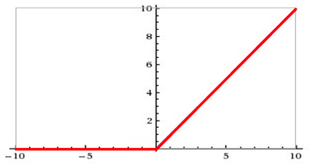
\includegraphics[width=\linewidth]{Images/ReLU.png}
     \caption{\label{fig:ReLU}ReLU.}
  \end{subfigure}
  \begin{subfigure}[b]{0.3\linewidth}
    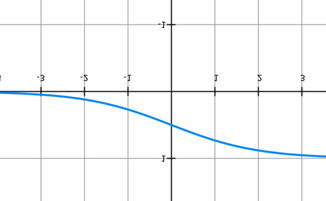
\includegraphics[width=\linewidth]{Images/Sigmoid.png}
    \caption{\label{fig:Sigmoid}Sigmoid.}
  \end{subfigure}
  \begin{subfigure}[b]{0.3\linewidth}
    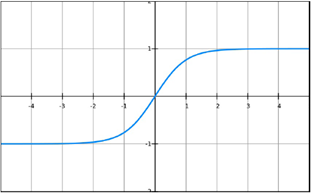
\includegraphics[width=\linewidth]{Images/Tanh.png}
    \caption{\label{fig:Tanh}Tanh.}
  \end{subfigure}
  \begin{subfigure}[b]{0.3\linewidth}
    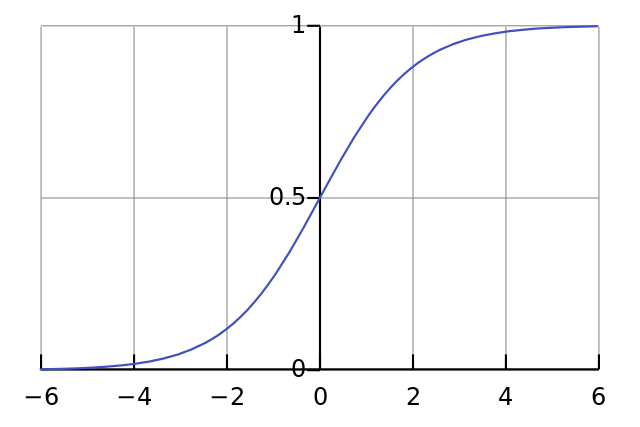
\includegraphics[width=\linewidth]{Images/Softmax.png}
     \caption{\label{fig:Softmax}Softmax.}
  \end{subfigure}
  \begin{subfigure}[b]{0.3\linewidth}
    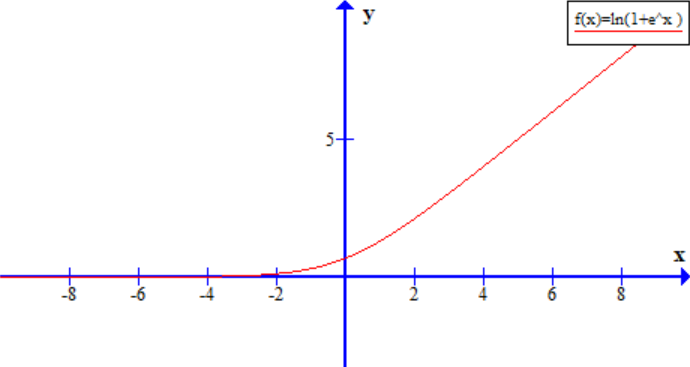
\includegraphics[width=\linewidth]{Images/Softplus.png}
    \caption{\label{fig:Softplus}Softplus.}
  \end{subfigure}
  \begin{subfigure}[b]{0.3\linewidth}
    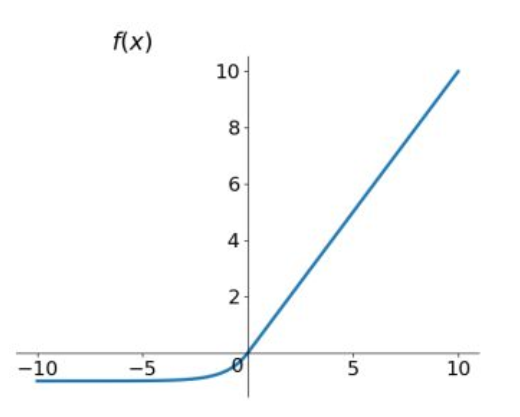
\includegraphics[width=\linewidth]{Images/ELU.png}
    \caption{\label{fig:ELU}ELU.}
  \end{subfigure}
  \caption{Six Activation Functions.}
  \label{fig:Activation Functions}
\end{figure}
\section{Three common types of Neural Network}
%
\subsection{Single-Layer Perceptron Neural Network}
Since the single-layer perceptron neural network is the simplest kind of neural network, it is necessary to cover it in report for better understanding the artificial neural network. A single-layer perceptron neural network consists of one input layer, which only transfers data, and one output layer. The neuron in output layer contains a threshold $\theta{}$. Meanwhile, for every connection in network, they have their own weight. The architecture of Single-Layer Perceptron is shown in Figure~\ref{fig:Perceptron_Neural_Network}.
\begin{figure}[h]
\centering
\fboxsep 2mm
\framebox{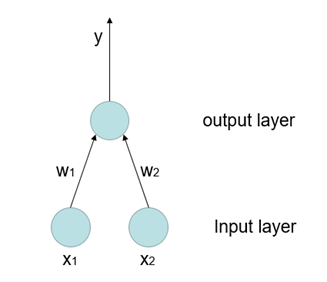
\includegraphics[width=6cm]{Images/Perceptron_Neural_Network.png}}
\caption{\label{fig:Perceptron_Neural_Network} Two-layer Perceptron Neural Network.}
\end{figure}
\\Perceptron neural networks use step function as activation function.
\begin{equation}
f\left(x\right)=\left\{\begin{array}{l}0,\ \ x<0 \\
\ 1,\ \ x\geq{}0\ \end{array}\right.
\end{equation}
Therefore, the output of neuron is: 
\begin{equation}
y=f\left(\sum_i{w_ix}_i-\theta{}\right)
\end{equation}
Replace the threshold with bias $b\ (b=-\theta{})$, so the output of the neural network is:
\begin{equation}
y=f\left(\sum_i{w_ix}_i+b\right)
\end{equation}
The weights and bias in perceptron can be trained by using a learning algorithm called the delta rule. For input training data $(x,\ y)$, if the output of neuron is $\hat{y}$, then we can adjust weights in this way:
\begin{equation}
w_i\leftarrow{}w_i+\Delta{}w_i
\end{equation}
\begin{equation}
\Delta{}w_i=\eta{}\left(y-\hat{y}\right)x_i
\end{equation}
Where $\eta{}\in{}(0,1)$ is called learning rate.
%
\subsection{Feedforward Neural Networks}
Feedforward neural network, also called multilayer perceptron (MLP), is a simple but very important type of neural network. In feedforward neural network, information directly moves from input layer to output layer through hidden layers without any cycles, which means there is no feedback connection. Both fully connected neural network and convolutional neural network developed in this project for image classification are feedforward neural networks.

The goal of a feedforward neural network is to approximate some function $f^*\hat{y}$, which can map an input $y$ to a category $y$. A feedforward neural network defines a mapping $y=f^*(x;\ \theta{})$ and learns the value of parameters $\theta{}$ that result in the best function approximation~\cite{Goodfellow:2000}. The training of feedforward neural network will be discussed later.
%
\subsection{Convolutional Neural Network}
Convolutional neural networks (CNN) is a kind of advanced model widely used in image classification. It can extract higher-level features from images and learn these features. Similar to the normal fully connected neural network, convolutional neural network consists of layers of neurons with weights and biases.

However, in normal fully connected neural network, each neuron in each layer is connected to every neurons in previous layer, which makes the number of weights in each layer will become very large especially in first hidden layer when the input images are big. For example, if the size of input images is 256*256*3, the first layer will need 196608 weights to scale the images. This will make the number of parameters dramatically increase. Meanwhile, because the neurons in each layer are independent to each other, it is impossible for them to share any connections, which means the information about object’s shape in image is partly wasted. 

To solve all of this problem, convolutional neural network have a very different architecture. Convolution neural network contain three kinds of layers: convolutional layer, polling layer and dense layer (fully connected layer). Each kind of layer have different features and functions. The overall architecture is shown in Figure~\ref{fig:The basic structure of Convolutional Neural Network}.
\begin{figure}[h]
\centering
\fboxsep 2mm
\framebox{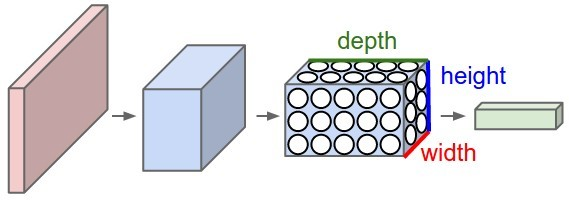
\includegraphics[width=6cm]{Images/The_basic_structure_of_Convolutional_Neural_Network.jpg}}
\caption{\label{fig:The basic structure of Convolutional Neural Network} The basic structure of Convolutional Neural Network.}
\end{figure}
\paragraph{Convolutional Layer}
The convolutional layer in CNN applies numbers of convolution filters to perform a set of calculations and extract information. For each sub-region, a filter will produce a value and save the value in the output feature map. Unlike the fully connected neural network, the neurons in convolutional layer are arranged in three dimensions (width, height and depth), and neurons in each layer are just connected to a small region of layer before it. Therefore, the number of parameters will be reduced.
\paragraph{Pooling Layer}
Polling layer will reduce the dimensionality of the feature map to improve the efficiency and performance of the classification by decrease the quantity of data. It will extract the maximum value from each sub-region and abandon others.
\paragraph{Fully connected layer (Dense layer)}
The dense layers is very similar to the layer of normal neural network. Every node in this layer is connected to every node in preceding layer.

A CNN model is usually comprise with a stack of convolution modules and several dense layers. Each convolutional module is composed of a convolutional layer and a following polling layer. Meanwhile, the dense layers are in charge of the classification. The number of nodes in the final dense layer is equal to the number of target classes.
%%%
\section{The Training of Feedforward Neural Network}
Since both fully connected neural network and convolutional network developed in this project are feedforward neural networks, it is necessary and important to know how to train a feedforward neural network. In this section, some important conceptions about the training are discussed.
%%
\subsection{Error Based Learning}
Feedforward neural network defines a mapping $y=f^*(x;\ \theta{})$, where x is input and y is output. To learn the parameters $\theta{}$, we need to make the output of neural network close to the actual value of input. This goal can be achieved by using loss function as objective function. The neural network will be trained by minimizing the value of loss function through training process, reducing the difference between predicted value and the actual value of the input.
%%
\subsection{Loss Function}
Loss function, or cost function, is a function used to quantify how close the output of a neural network is to the actual input. It can efficiently measure how good the network is by analyzing the difference between predictions form input and the truth. The cross-entropy is a widely used loss function and we used this function in all of our experiments in this project.
Cross-entropy:
\begin{equation}
H\left(p,q\right)=-\sum q_i\log{\left(p_i\right)}
\end{equation}
Where $p$ is the actual probabilities and $q$ is the computed probability.
%%
\subsection{Gradient Descent}
Gradient descent is an algorithm for finding the local minimum of a function. It is a very popular in the training of neural networks since it is good at minimizing the loss function. For the gradient of a function at a certain point, the direction of gradient is the direction where the value of function will increase fastest, while the value of gradient is the biggest directional derivative (or slope in two-dimension word). Therefore, to minimize the loss function, we can take a step in the opposite direction to the gradient, where the loss function decrease fastest. The size of the step is called learning rate. For better explaining the gradient descent, here is an example:

The simple neural network as shown in Figure~\ref{fig:Feedforward_Neural_Network} below consists of two layers. However, only the output layer contains functional neurons, and the input layer is just for transmitting.
\begin{figure}[h]
\centering
\fboxsep 2mm
\framebox{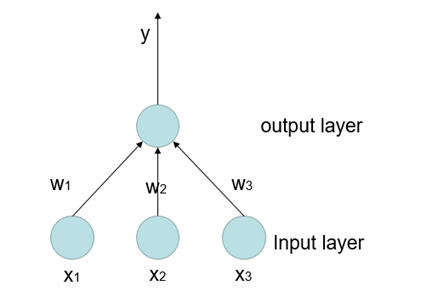
\includegraphics[width=6cm]{Images/Feedforward_Neural_Network.png}}
\caption{\label{fig:Feedforward_Neural_Network} Simple Neural Network.}
\end{figure}
\\Assume the neuron in output layer does a weighted sum of all of its inputs and adds a bias b, and Softmax is used as activation function. The output of a neuron is:
\begin{equation}
y=softmax\left(\sum_i{w_ix}_i+b\right)
\end{equation}
For a training data $(x,y)$. Assume the output of the neural network is $\hat{y}$. Use cross-entropy as loss function. We can get:
\begin{equation}
E=ylog\left(\hat{y}\right)
\end{equation}
Starting with some initial value of weights and bias, we can obtain gradient by computing the partial derivatives of the loss function relatively to all the weights and biases. Then update the parameters with learning rate $\eta{}$:
\begin{equation}
w_i\leftarrow{}w_i+\Delta{}w_i
\end{equation}
\begin{equation}
\Delta{}w_i=\eta{}\frac{\partial{}E}{\partial{}w_i}
\end{equation}
%%
\subsection{Backpropagation}
Backpropagation or Error Back Propagation is one of the most popular learning techniques in training multi-layer neural network. Backpropagation allows the information flow backwards through the network, in order to compute the gradient. For example, there is a three-layer feedforward neural network as shown in Figure~\ref{fig:Multi_Feedforward_Neural_Network} below. There are d neurons in first layer, q neurons in hidden layer, and l neurons in output layer. The thresholds of hidden-layer and output-layer neurons are as γ and θ respectively. Assume all of the hidden and output layer neurons are using Sigmoid as activation function.
\begin{figure}[h]
\centering
\fboxsep 2mm
\framebox{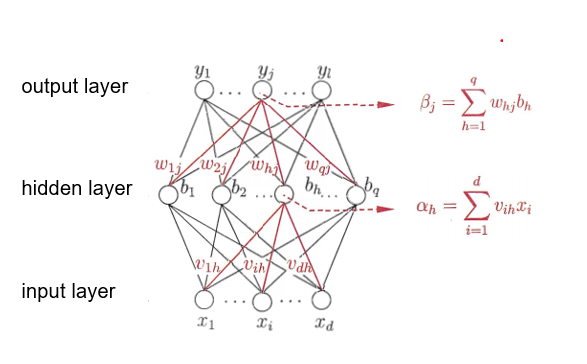
\includegraphics[width=6cm]{Images/Multi_Feedforward_Neural_Network.png}}
\caption{\label{fig:Multi_Feedforward_Neural_Network} Multi Feedforward Neural Network~\cite{Zhou:2016}.}
\end{figure}
\\For training data $(x_k,y_k)$, assume the output of neural network is
${\hat{y}}_k=({\hat{y}}_1^k{,\ \hat{y}}_2^k,{\hat{y}}_3^k,…,{\hat{y}}_l^k)$.
\begin{equation}
{\hat{y}}_j^k=f({\beta{}}_j-{\theta{}}_j)
\end{equation}
Then we can calculate the squared error according to the actual input and the output (this is just an example, different loss functions can be used here).
\begin{equation}
E_{k=}\frac{1}{2}\sum_{j=1}^l{({\hat{y}}_j^k-{\hat{y}}_j^k)}^2
\end{equation}
To update a parameter $v$ after each iteration, the formula should be:
\begin{equation}
v\leftarrow{}v+\Delta{}v
\end{equation}
Calculate the partial derivative of the error with respect to a weight $w_{hj}$ by using the chain rule.
\begin{equation}
\frac{\partial{}E_k}{\partial{}w_{hj}}=\frac{\partial{}E_k}{\partial{}{\hat{y}}_j^k}\cdot{}\frac{\partial{}{\hat{y}}_j^k}{\partial{}{\beta{}}_j}\cdot{}\frac{\partial{}{\beta{}}_j}{\partial{}w_{hj}}
\end{equation}
Finally, update the parameter with learning rate $\eta{}$. For $w_{hj}$:
\begin{equation}
w_{hj}\leftarrow{}w_{hj}+\Delta{}w_{hj}
\end{equation}
\begin{equation}
\Delta{}w_{hj}=\eta{}\frac{\partial{}E_k}{\partial{}w_{hj}}
\end{equation}
%%%%%%%%%%%%%%%%%%%%%%
%%% The Classification of MNIST hand written digital images
\chapter{\label{chapter3}The Classification of MNIST hand written digital images}
\section{Introduction}
Hand writing digits recognition is a classical problem in image classification. The purpose of this experiment is to solve this problem by using the technology of Artificial Neural Network. The MNIST database used in this experiment contains 70,000 labelled handwritten digits, 60,000 for training and 10,000 for test. This database is come from the source\footnote{\url{http://yann.lecun.com/exdb/mnist/}.}.

To classify these images, two different kinds of neural network models were build. One is a fully-connected neural network, and the other is a convolutional neural network. The process of the building and training these two models will be introduced respectively in this chapter.
\subsection{Technique}
In this experiment, all the codes are written in Python, and TensorFlow is imported in to program as library. TensorFlow is an open source software library for numerical computation using data-flow graphs, it has been widely used for machine learning and artificial neural network research. 
\subsection{Experiment Environment}
\begin{itemize}
\item {\sl Computer Model:} Lenovo IdeaPad 700s
\item {\sl Processor:} Intel(R) Core(TM) m7-6Y75 1.20GHz
\item {\sl RAM:} 8.00 GB.
\item {\sl OS:} Windows 10.
\end{itemize}
%3.4
\section{Classifying Handwritten Digits Images with Fully-connected Neural Network Model}
To build a fully-connected neural network for solving this problem, at the beginning, a simple one layer neural network was established. Then, the key features of this neural network, which can affect the performance of the neural network, will be adjusted, aiming to improve the accuracy of the classification. This experiment contains four scenarios. In each scenario, one of the neural network’s features (including the number of layers, the usage of activation function and the usage of extra techniques) will be changed, while the others remain unchanged. Each experiment in these four scenario lasts 4 epochs and each epoch contains 600 training iterations and 100 test iterations. The batch size of the test and training dataset in each iteration are both 100.
%3.4.1
\subsection{Scenario 1: Implement a sample one-layer neural network and test different activation functions}
Activation function plays an important role in neural network. Because the most suitable activation functions in neural network for different problems in our real life are not always the same, finding the most suitable activation functions become a necessary way to improve the performance. 

The development of the suitable fully-connected neural network for this problem starts from a sample one-layer neural network. Since this neural network only contains one layer, which is actually the output layer, to find the most suitable activation function in output layer for this problem among all the six activation functions mentioned in background research, this scenario will contain three experiments, and the model in each experiment will using different activation functions, while other parameters remain unchanged.

The reason why we did not test all six activation functions introduced in background research in this scenario is that some of the functions will produce zero or negative value, which are undesired for this one layer model, and it will lead to failure.

Common features of the neural networks in this scenario:
\begin{itemize}
\item {\sl Loss Function:} cross-entropy
\item {\sl Learning Rate:} 0.003
\end{itemize}
\subsubsection{Experiment 1: using Softmax}
In this experiment, Softmax is used as activation function.
\begin{figure}[h]
\centering
\fboxsep 2mm
\framebox{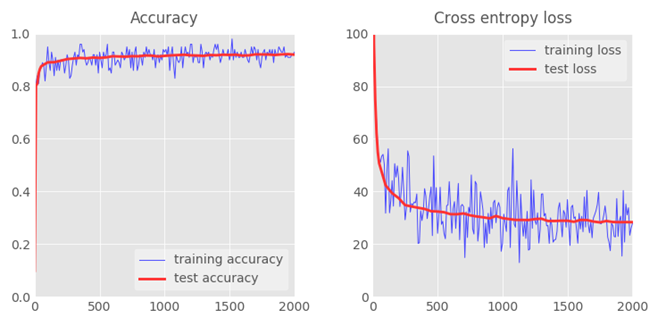
\includegraphics[width=6cm]{Images/MNIST_fully_coneected_S1E1.png}}
\caption{\label{fig:MNIST_fully_coneected_S1E1} The performance of simple 1-layer neural network using Softmax as activation function}
\end{figure}
\\Result: The result of this experiment, as shown in Figure~\ref{fig:MNIST_fully_coneected_S1E1} above, clearly shows that both training and test accuracy of the model dramatically increased from zero to about 0.9 at the very beginning and then climb slowly as the increase of iterations. Meanwhile the values of training loss and test loss decreased from 100 to about 30. After 2000 times of iterations, this model achieved an accuracy of 0.9222, which is not bad for a one layer simple neural network. The blue lines represent the training results and the red lines represent the test results.

However, for utilizing or solving a problem in the real world, a model with such accuracy it is not good enough. To improve the performance of the neural network model, in next steps, some other activation functions will be tested, replacing the Softmax function in this model.
\subsubsection{Experiment 2: using Sigmoid}
Sigmoid is another common activation function in neural network. To test if sigmoid can improve the performance, in this experiment, sigmoid will be used as activation function while the rest of the code is unchanged. 
\begin{figure}[h]
\centering
\fboxsep 2mm
\framebox{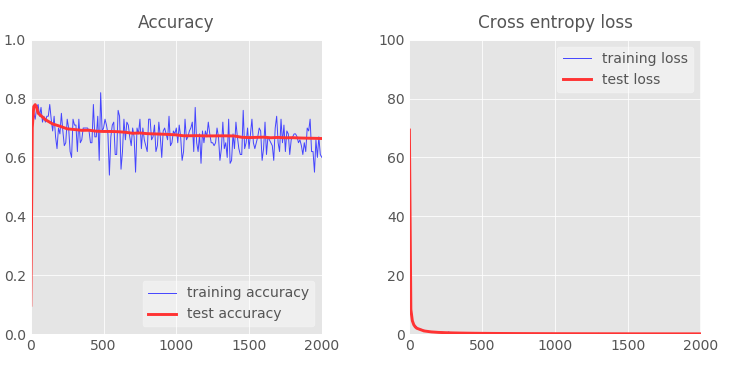
\includegraphics[width=6cm]{Images/MNIST_fully_coneected_S1E2.png}}
\caption{\label{fig:MNIST_fully_coneected_S1E2} The performance of simple 1-layer neural network using Sigmoid as activation function}
\end{figure}
\\Result: The result is shown in Figure~\ref{fig:MNIST_fully_coneected_S1E1} above. The accuracy increased to about 0.78 rapidly at the beginning, and then slowly decreased to about 0.68. Meanwhile the cross entropy loss rapidly decreases to about zero and then stabilize at that value. The performance of this model is not as good as the last model with Softmax. 
\subsubsection{Experiment 3: using Softplus}
In this experiment, Softplus is used as activation function. . 
\begin{figure}[h]
\centering
\fboxsep 2mm
\framebox{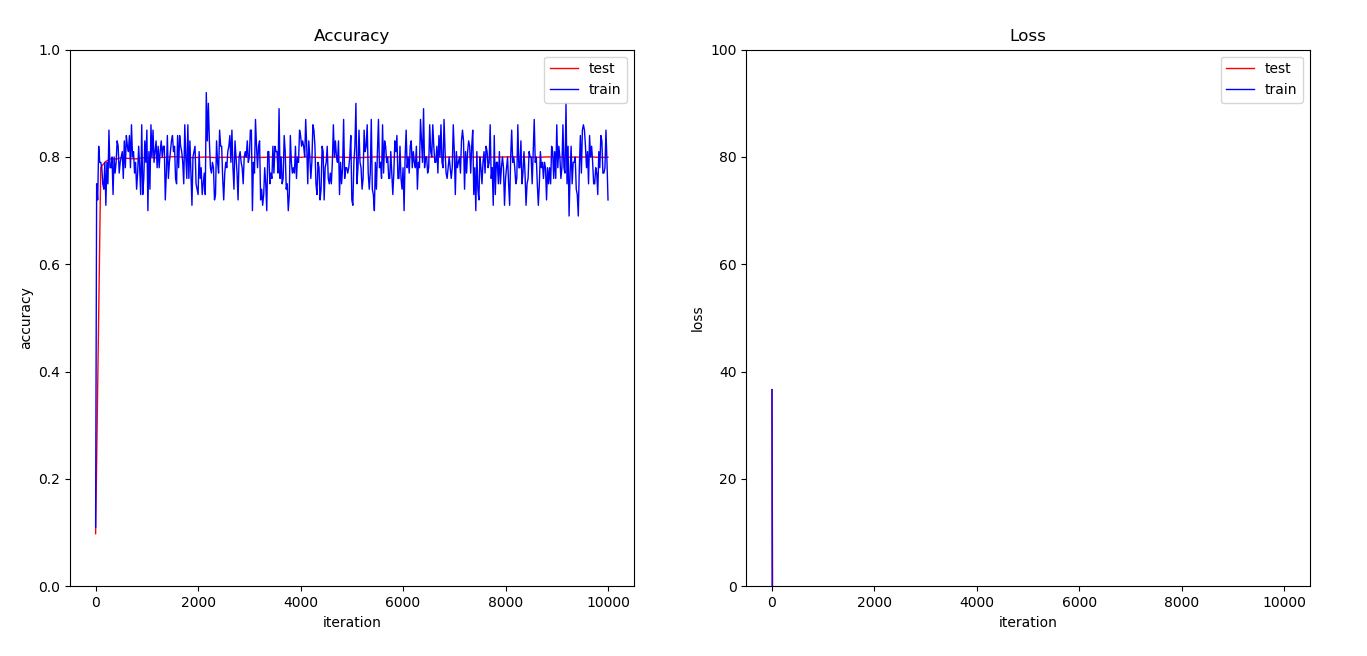
\includegraphics[width=6cm]{Images/MNIST_fully_coneected_S1E3.png}}
\caption{\label{fig:MNIST_fully_coneected_S1E3} The performance of simple 1-layer neural network using Softplus as activation function}
\end{figure}
\\Result: The result is shown in Figure~\ref{fig:MNIST_fully_coneected_S1E3} above. This model achieved an accuracy of 0.7995. The performance of this model is better than Sigmoid, but worse than Softmax.
\subsubsection{Summary}
According to the results of these experiments, it is notable that the usage of different activation functions can significantly affect the performance of neural network model. However, in this case, without changing other configurations, using the Softmax function as activation function can let this simple 1-layer neural network model gets a better performance. So in the following experiments, the Softmax will be used as activation function in output layer.
%3.4.2
\subsection{Scenario 2: Adding more layers into the neural network model}
In neural network, more layers usually means more trainable weights and biases. With more trainable parameters in model, more information can be deposited in the neural network, which can help in improving the performance of the classifier.

In this scenario, based on the simple 1-layer neural network established in experiment 1 Scenario 1, one to more layers will be added into the model as hidden layers to improve its performance. According to the previous experiments, the Softmax is the most suitable function for one-layer neural network among six activation functions introduced in background research, so all the neuron network models in this scenario will use Softmax as output layer activation function.

However, the suitable activation function in hidden layers still need to be found through experiments. In this scenario, at first, a two-layer neural network with Softmax used in both layers will be established, and then different activation functions will be tested in first layer (input layer). When the most suitable activation function among the six functions is found, more layers will be added into the model with this function as the activation function.

Common features of the neural networks in this scenario:
\begin{itemize}
\item {\sl Activation function:} Softmax in output layer
\item {\sl Loss Function:} cross-entropy
\item {\sl Learning Rate:} 0.003
\end{itemize} 
%
\subsubsection{Experiment 1: using Softmax in input layer}
Adding one layer into the 1-layer neural network and observe its performance. Using Softmax as activation function in this new layer (input layer).
\begin{figure}[h]
\centering
\fboxsep 2mm
\framebox{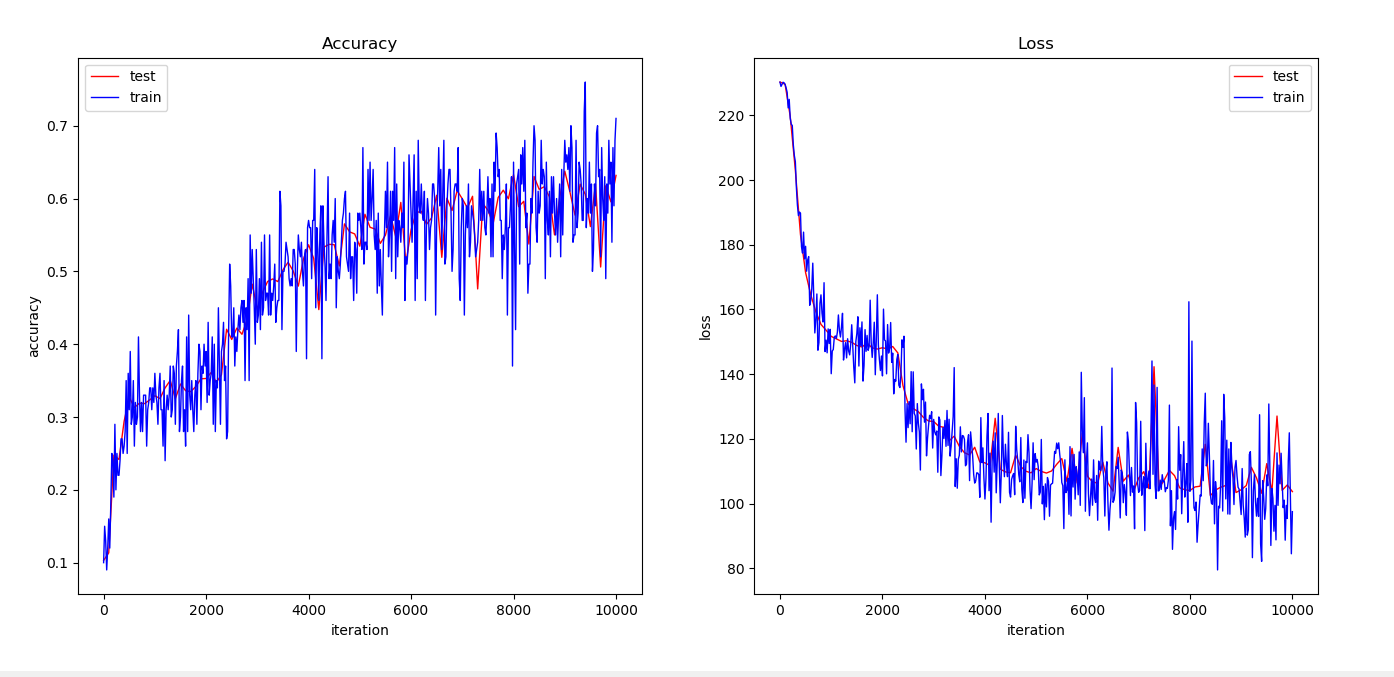
\includegraphics[width=6cm]{Images/MNIST_fully_coneected_S2E1.png}}
\caption{\label{fig:MNIST_fully_coneected_S2E1} The performance of 2-layer neural network using Softmax in input layer}
\end{figure}
\\Result: The result is shown in Figure~\ref{fig:MNIST_fully_coneected_S2E1} above. This model achieved an accuracy of 0.6376. The performance of this model is worse than the 1-layer neural network using Softmax (in experiment 1 scenario 1), whose accuracy is 0.9222.
%
\subsubsection{Experiment 2: using ReLU in input layer}
Replace the Softmax in first layer with ReLU.
\begin{figure}[h]
\centering
\fboxsep 2mm
\framebox{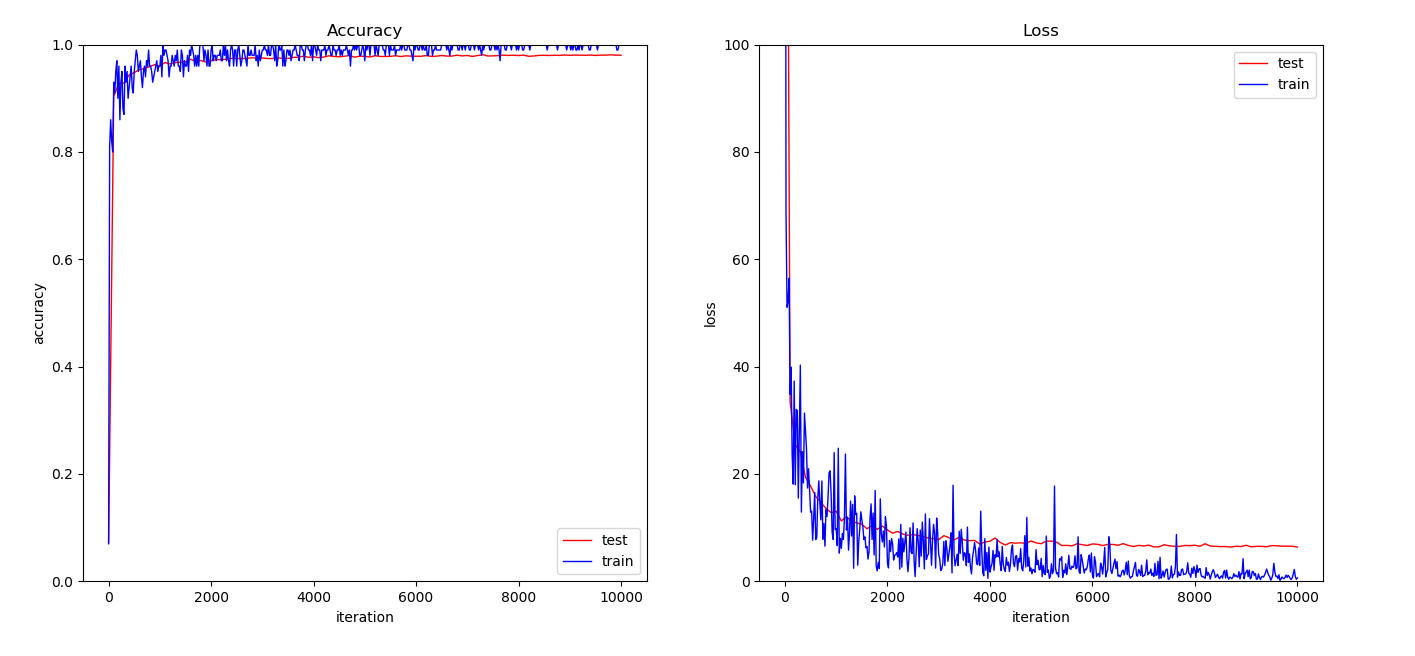
\includegraphics[width=6cm]{Images/MNIST_fully_coneected_S2E2.png}}
\caption{\label{fig:MNIST_fully_coneected_S2E2} The performance of 2-layer neural network using ReLU in input layer}
\end{figure}
\\Result: The performance of this model is shown in Figure~\ref{fig:MNIST_fully_coneected_S2E2} above. The accuracy is 0.9814 and the loss is 6.3856. Compared with the original one-layer model’s accuracy 0.9222, clearly the performance of this model is better.
%
\subsubsection{Experiment 3: using Sigmoid in input layer}
Using Sigmoid as activation function in first layer.
\begin{figure}[h]
\centering
\fboxsep 2mm
\framebox{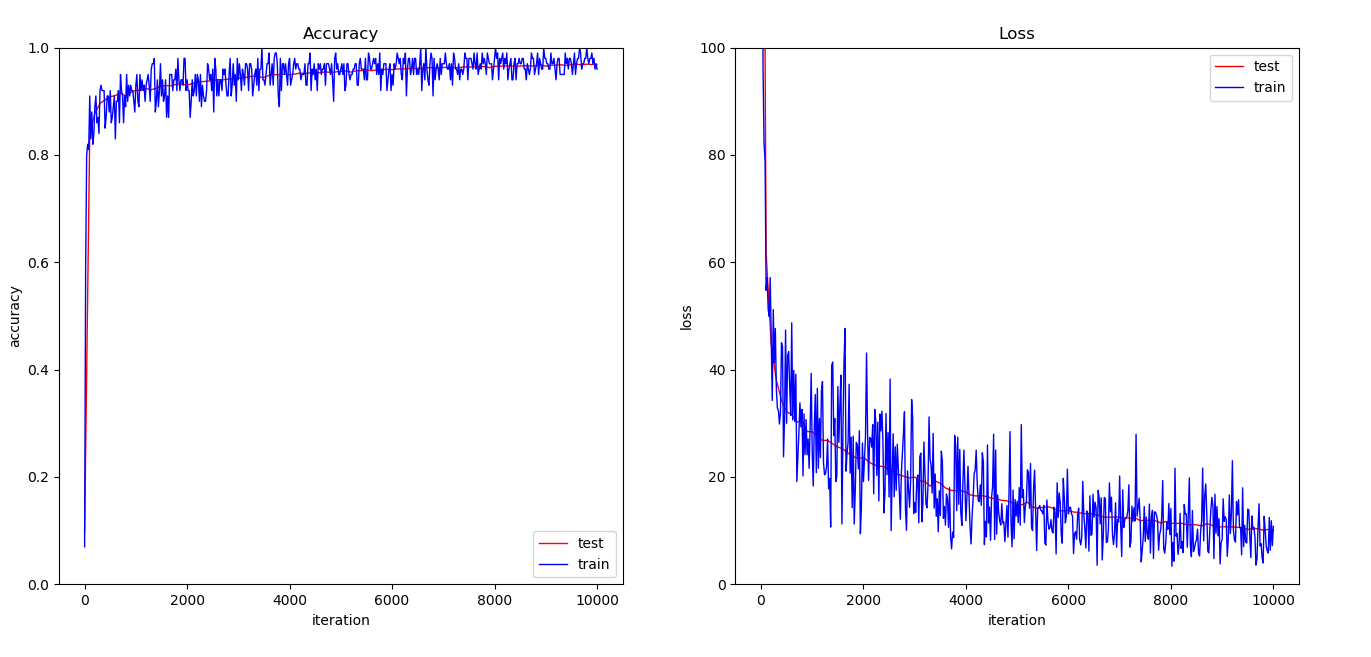
\includegraphics[width=6cm]{Images/MNIST_fully_connected_S2E3.png}}
\caption{\label{fig:MNIST_fully_connected_S2E3} The performance of 2-layer neural network using Sigmoid in input layer}
\end{figure}
\\Result: The performance of this model is shown in Figure~\ref{fig:MNIST_fully_connected_S2E3} above. The accuracy is 0.9693 and the loss is 10.0908. The performance of this model is better than original one-layer model but worse than the two-layer model using Relu in first layer.. 
%
\subsubsection{Experiment 4: using Tanh in input layer}
Using Tanh as activation function in first layer.
\begin{figure}[h]
\centering
\fboxsep 2mm
\framebox{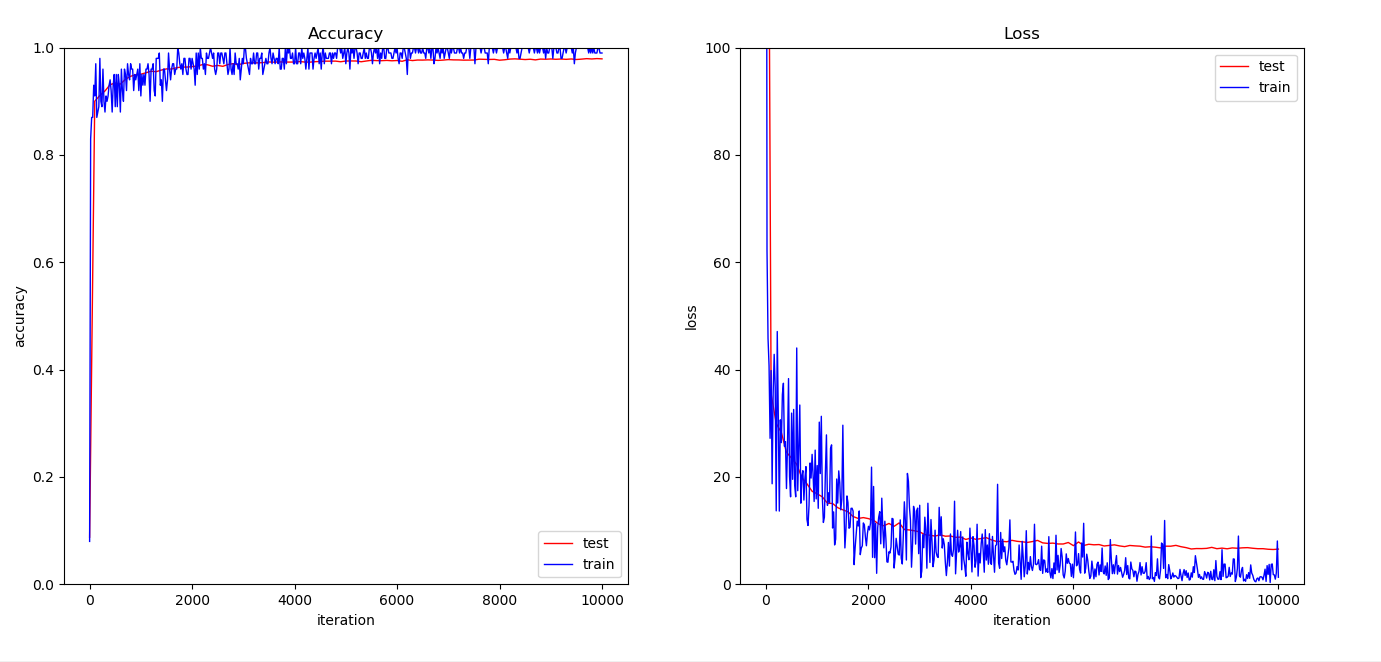
\includegraphics[width=6cm]{Images/MNIST_fully_connected_S2E4.png}}
\caption{\label{fig:MNIST_fully_connected_S2E4} The performance of 2-layer neural network using Tanh in input layer}
\end{figure}
\\Result: The performance of this model is shown in Figure~\ref{fig:MNIST_fully_connected_S2E4} above. The  accuracy is 0.9796 and the loss is 6.48982. The performance of this model is better than last experiment but worse than the model using Relu.
%
\subsubsection{Experiment 5: using ELU in input layer}
Using ELU as activation function in first layer.
\begin{figure}[h]
\centering
\fboxsep 2mm
\framebox{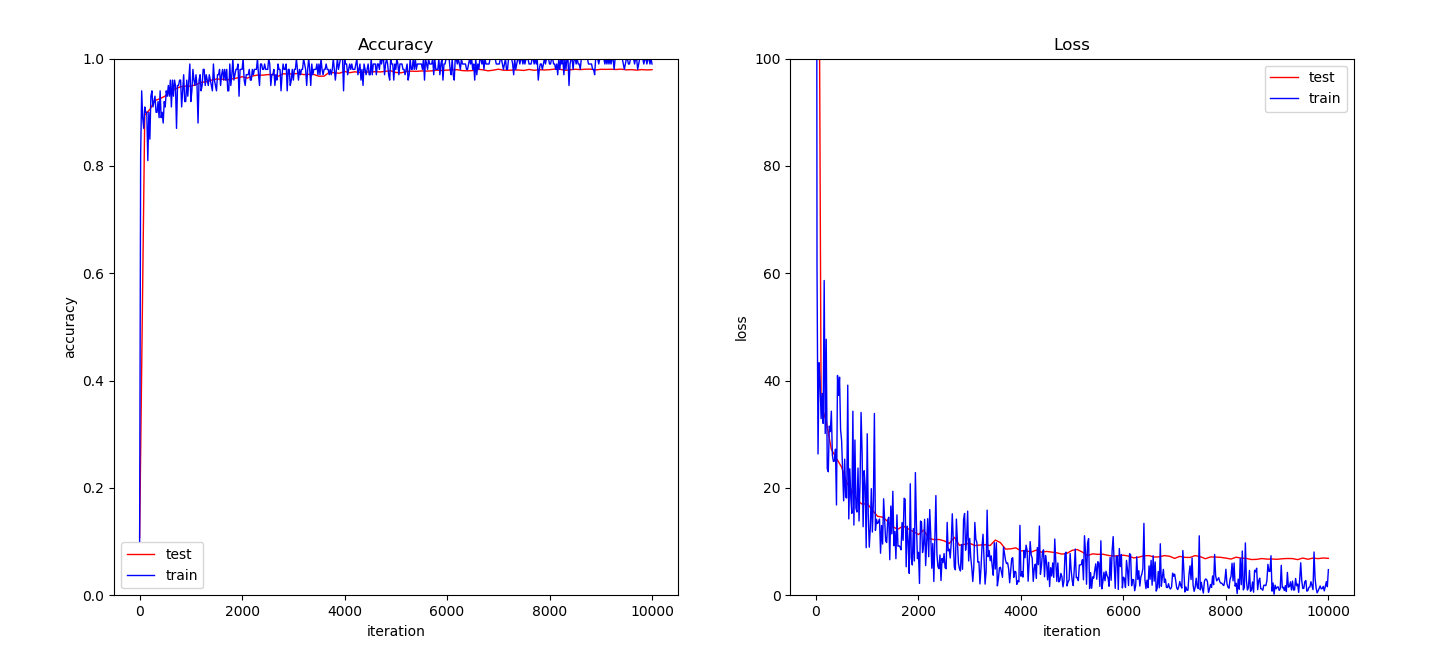
\includegraphics[width=6cm]{Images/MNIST_fully_connected_S2E5.png}}
\caption{\label{fig:MNIST_fully_connected_S2E5} The performance of 2-layer neural network using Tanh in input layer}
\end{figure}
\\Result: The performance of this model is shown in Figure~\ref{fig:MNIST_fully_connected_S2E5} above. The maximum accuracy is 0.9805 and the minimum loss is 6.65515.
%
\subsubsection{Experiment 6: using Softplus in input layer}
Using Softplus as activation function in first layer.
\begin{figure}[h]
\centering
\fboxsep 2mm
\framebox{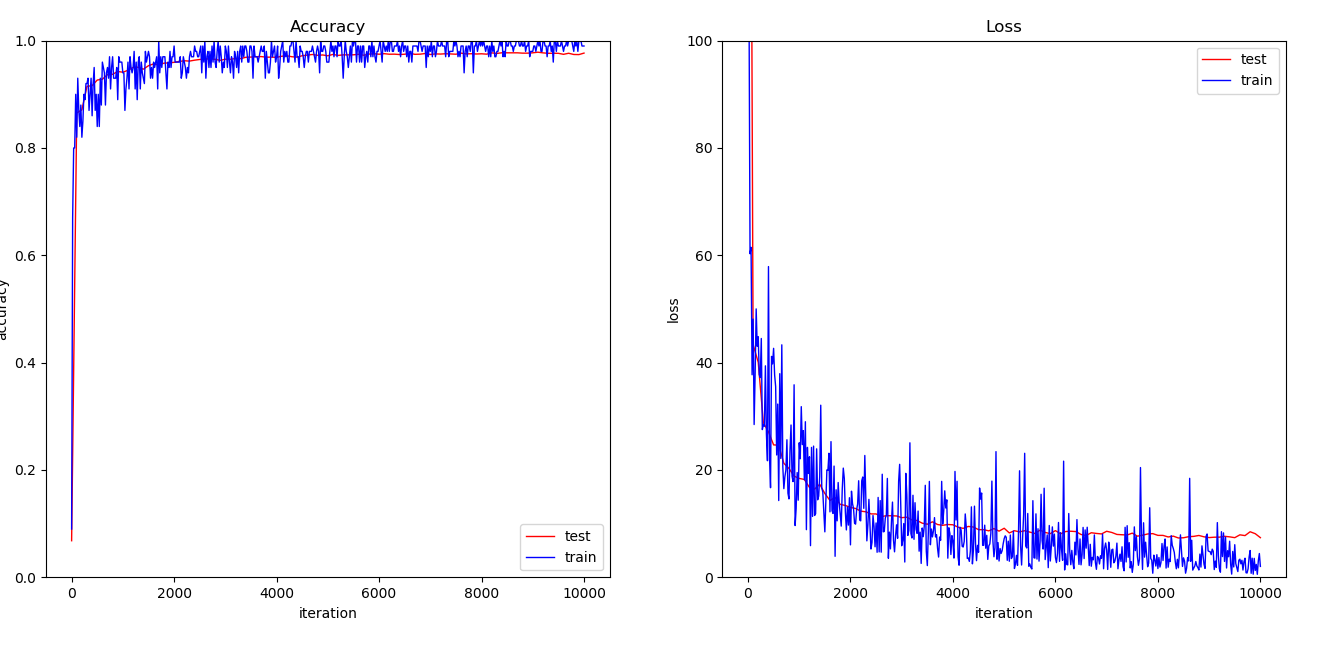
\includegraphics[width=6cm]{Images/MNIST_fully_connected_S2E6.png}}
\caption{\label{fig:MNIST_fully_connected_S2E6} The performance of 2-layer neural network using Softplus in input layer}
\end{figure}
\\Result: The performance of this model is shown in Figure~\ref{fig:MNIST_fully_connected_S2E6} above. The accuracy is 0.9785 and the loss is 7.33077.
%
\subsubsection{Result Summary}
According to the experiment results in Table~\ref{tab:table_1}, it is clear that the ReLU is the most suitable activation function in input layer for this problem. Since it is very common to use same activation function in input and hidden layers, in following experiments the ReLU will be used in both input and hidden layers.
\begin{table}[h!]
  \begin{center}
    \caption{Summary of experiment results (1 - 6).}
    \label{tab:table_1}
    \begin{tabular}{l|c|c}
      \textbf{Activation Function} & \textbf{Accuracy} & \textbf{Loss}\\
      \hline
      Softmax-Softmax model & 0.6376 & 102.472\\
      ReLU-Softmax model & 0.9814 & 6.3856\\
      Sigmoid-Softmax model & 6.3856 & 10.0908\\
      Tanh-Softmax model & 0.9796 & 6.48982\\
      ELU-Softmax model & 0.9805 & 6.65515\\
      Softplus-Softmax model & 0.9785 & 7.33077\\
    \end{tabular}
  \end{center}
\end{table}
%
\subsubsection{Experiment 7 - 9: Adding more layers into the model as hidden layer}
In experiment 7, 8 and 9, based on the two-layer model in Experiment 2, one to three hidden layer are added. The summary of experiment results is shown in Table~\ref{tab:table_2} below. Because the plots of this three experiment are very similar to Experiment 2, here they will be omitted.
\begin{table}[h!]
  \begin{center}
    \caption{Summary of experiment results (7 - 9).}
    \label{tab:table_2}
    \begin{tabular}{c|l|c|c}
      \textbf{NO.} &\textbf{Activation Function} & \textbf{Accuracy} & \textbf{Loss}\\
      \hline
      Experiment 7 & Three-layer model & 0.9826 & 6.37127\\
      Experiment 8 & Four-layer model & 0.9815 & 7.43263\\
      Experiment 9 & Five-layer model & 0.9811 & 8.11888\\
    \end{tabular}
  \end{center}
\end{table}
According to these results, it is notable that the performance of three-layer model is better than two-layer model in Experiment 2. However, with the increase of layers, the performance decreases. 

Observing the loss curves of these three experiments, as shown in Figure~\ref{fig:The noises of three different models} below, it is clear that the noise grew with the number of the layers, and the test loss of five-layer model slightly increased after about 2000 iterations while the training loss continually declined. This phenomenon is what we called “overfitting”. In following scenarios, we implemented some useful mechanisms to solve these problems.
\begin{figure}[h]
\centering
\fboxsep 2mm
\framebox{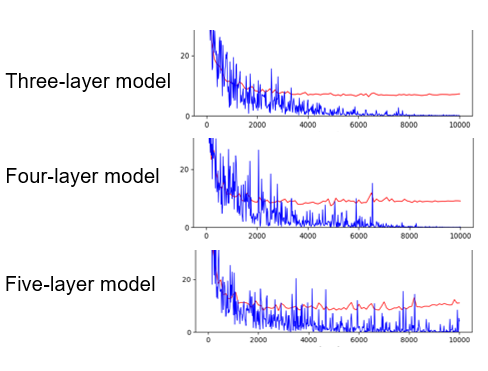
\includegraphics[width=6cm]{Images/The_increase_of_noise.png}}
\caption{\label{fig:The noises of three different models} The noises of three different models}
\end{figure}
%3.4.3
\subsection{Scenario 3: Implement learning rate decay into model}
To reduce the noise appeared in Figure~\ref{fig:The noises of three different models}, in this scenario, a technique called learning rate decay will be implemented. Through decreasing the learn rate of the neural network during the training process, the fluctuation of accuracy and loss will shrink. The neural network in this scenario is based on the five-layer model established in experiment 9 scenario 2, and the learning rate will decay from 0.003 to 0.0001 during the training process. 

Other features of the neural networks in this scenario:
\begin{itemize}
\item {\sl Number of Layers:} 5
\item {\sl Activation function:} Softmax in output layer and ReLU in input and hidden layers
\item {\sl Loss Function:} cross-entropy
\end{itemize} 
Result: The performance of this model is shown in Figure~\ref{fig:MNIST_fully_connected_S3E1} below. The accuracy is 0.9835 and the loss is 7.6305. After implemented the learning rate decay mechanism, the noises of both accuracy and loss curves are reduced. Meanwhile, the accuracy also improved from 0.9811 to 0.9835. Because of the good performance of this model, the technique of learning rate decay will be used in following experiments. 
\begin{figure}[h]
\centering
\fboxsep 2mm
\framebox{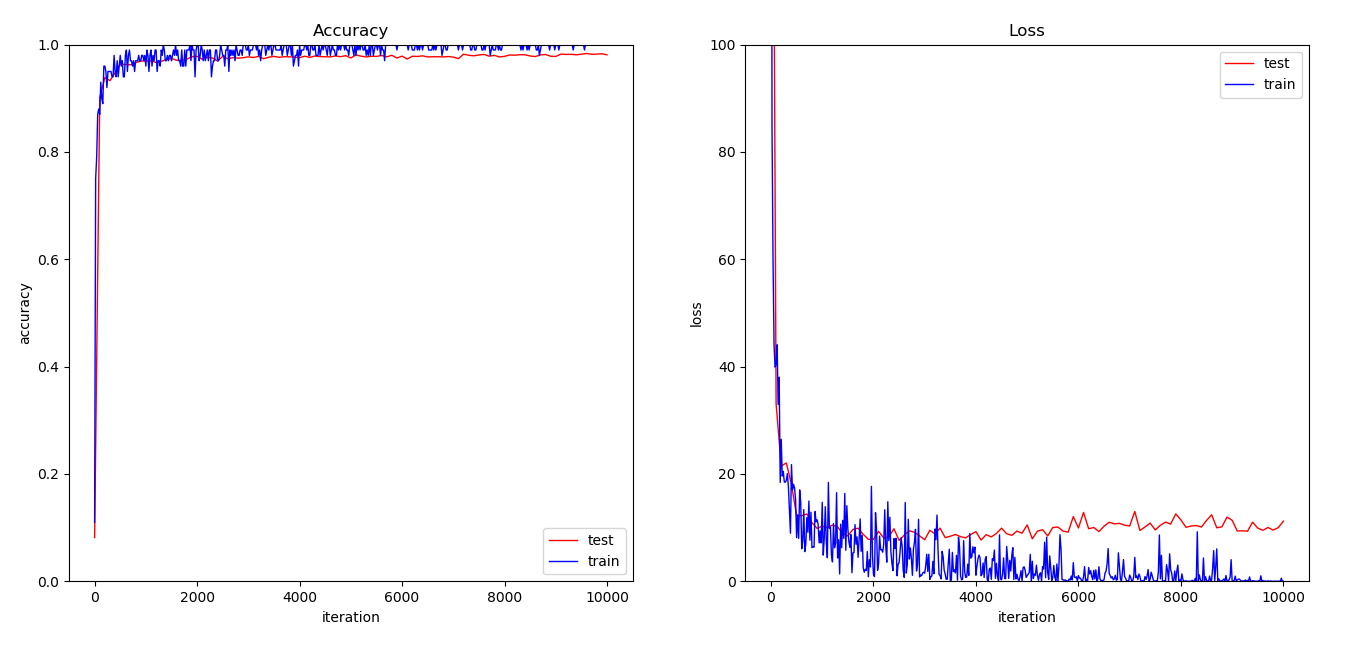
\includegraphics[width=6cm]{Images/MNIST_fully_connected_S3E1.png}}
\caption{\label{fig:MNIST_fully_connected_S3E1} The performance of the five-layer model implemented learning rate decay}
\end{figure}
%3.4.4
\subsection{Scenario 4: Implement neuron dropout into model}
Observing the result of scenario 3, as shown in Figure~\ref{fig:MNIST_fully_connected_S3E1}, the problem of overfitting is a little bit lighter than previous experiments. However, the problem is still exist.

Dropout is a useful measure in preventing overfitting in machine learning and deep learning. In this scenario, to prevent overfitting, dropout will be implemented in to the output layer of the model. The neural network will randomly drop some neurons during the training process to makes the backpropagation process different even with same data batch. The neural network in this scenario is based on the model in scenario 3.

Other features of the neural networks in this scenario:
\begin{itemize}
\item {\sl Number of Layers:} 5
\item {\sl Activation function:} Softmax in output layer and ReL in input and hidden layers
\item {\sl Loss Function:} cross-entropy
\item {\sl Learning Rate: } decrease from 0.003 to 0.0001 gradually
\end{itemize} 
Result: The performance of this experiment is shown in figure ~\ref{fig:MNIST_fully_connected_S4E1}. The accuracy is 0.9835 and the loss is 7.80113. Compared with the result in last scenario, the overfitting problem has been relieved. The overall performance of this model is better than the model without node dropout mechanism. However, the maximum accuracy did not change. In consideration of its benefit, node dropout mechanism will be kept in model.
\begin{figure}[h]
\centering
\fboxsep 2mm
\framebox{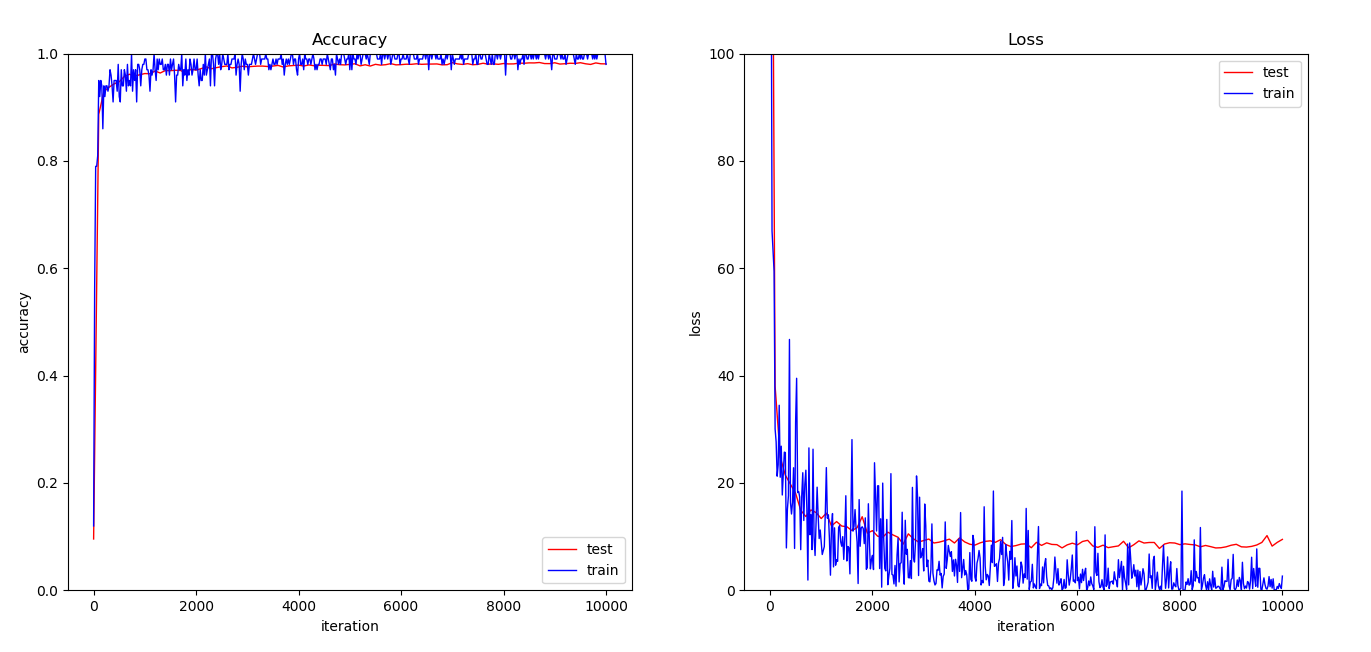
\includegraphics[width=6cm]{Images/MNIST_fully_connected_S4E1.png}}
\caption{\label{fig:MNIST_fully_connected_S4E1} The performance of the five-layer model implemented node dropout.}
\end{figure}
The model in this experiment is the best fully-connected neural network model build in this project for the classification of MNIST labelled  handwritten digits images.
%3.5%%%%%%%%%%%%%%%%%%%%%%%%
\section{Classifying Handwritten Digits Images with Convolutional Neural Network Model}
For the classification of handwritten digits images, the Convolutional Neural Network is a very successful model in solving this problem. This section will introduce the process of how we develop and train a convolutional neural network model for classifying the labelled handwritten digits images in MNIST database. 

First, a simple convolutional neural network was established. Then, we improved this model by changing the key parameters of this convolutional neural network, such as activation function, pooling activation, the number of layers, and using some useful techniques. This Experiment contains five scenarios, in each scenario, one of neural network's parameter will be changed, or one new technique will be used in model while other features remain unchanged. The training process in each experiment will last 4 epochs and each epoch contains 500 iterations.  The batch size for train set and test set are both 100.
%3.5.1
\subsection{Implement a sample convolutional neural network model with different activation functions in convolutional layer and dense layer}
Activation function is a very component in neural network. For different real problems, the suitable activation function are usually different. In this scenario, six popular activation functions mentioned previously were tested. According to the result of experiments, choose one suitable activation function to use in further experiments. 

The simple convolutional neural network model used in this scenario consists of one convolutional layer, one pooling layer and two fully connected layers (one dense layer and one logits layer). In this scenario, the activation function of convolutional layer and dense layer will be changed in each experiment and other features remain unchanged. The logits layer (the last layer) contains 10 Softmax neurons corresponding to 10 classes. The architecture of this convolutional neural network is shown in Figure~\ref{fig:MNIST_CNN_S1_Architecture}. 
\begin{figure}[h]
\centering
\fboxsep 2mm
\framebox{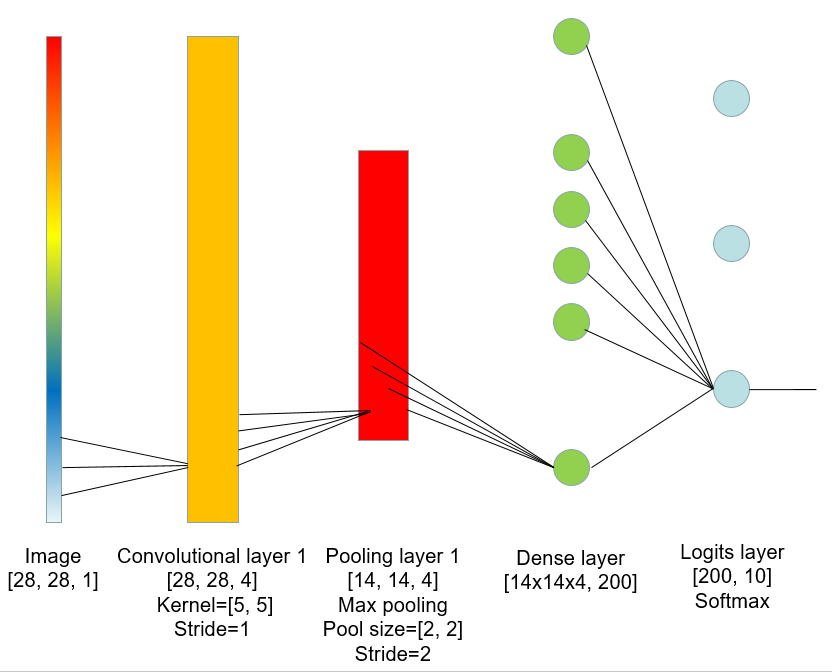
\includegraphics[width=6cm]{Images/MNIST_CNN_S1_Architecture.png}}
\caption{\label{fig:MNIST_CNN_S1_Architecture} The architecture of the convolutional neural network in this Scenario.}
\end{figure}
\\Common features of the neural networks in this scenario:
\begin{itemize}
\item {\sl Number of layers: } 4
\item {\sl Activation Function in logits layer:} Softmax
\item {\sl Pooling Function:} Max pooling
\item {\sl Loss Function:} cross-entropy
\item {\sl Learning Rate: } 0.003
\end{itemize}
%
\subsubsection{Experiment 1: using ReLU}
In this experiment, Rule is used as activation function in convolutional layer and dense layer.
\begin{figure}[h]
\centering
\fboxsep 2mm
\framebox{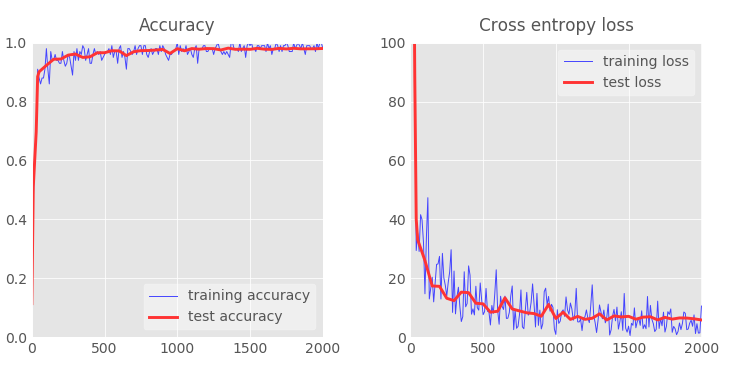
\includegraphics[width=6cm]{Images/MNIST_CNN_S1E1.png}}
\caption{\label{fig:MNIST_CNN_S1E1} The performance of convolutional neural network model using ReLU.}
\end{figure}
\\Result: the performance of this model is shown in Figure~\ref{fig:MNIST_CNN_S1E1}. This model achieved a accuracy of 0.9816, and the loss is 5.7996.
%
\subsubsection{Experiment 2: using Sigmoid}
In this experiment, Sigmoid replaced the ReLU in Experiment 1.
\begin{figure}[h]
\centering
\fboxsep 2mm
\framebox{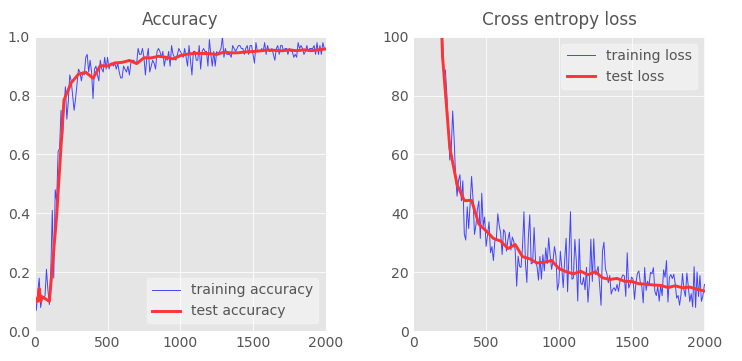
\includegraphics[width=6cm]{Images/MNIST_CNN_S1E2.png}}
\caption{\label{fig:MNIST_CNN_S1E2} The performance of the convolutional neural network model using Sigmoid.}
\end{figure}
\\Result: the result of this experiment is shown in Figure~\ref{fig:MNIST_CNN_S1E2}. The accuracy is 0.9585, and the test loss: 13.5983. It is obviously that the performance of this model is not as good as the model using ReLU. 
%
\subsubsection{Experiment 3: using Softmax}
In this experiment, Softmax is used as activation function.
\begin{figure}[h]
\centering
\fboxsep 2mm
\framebox{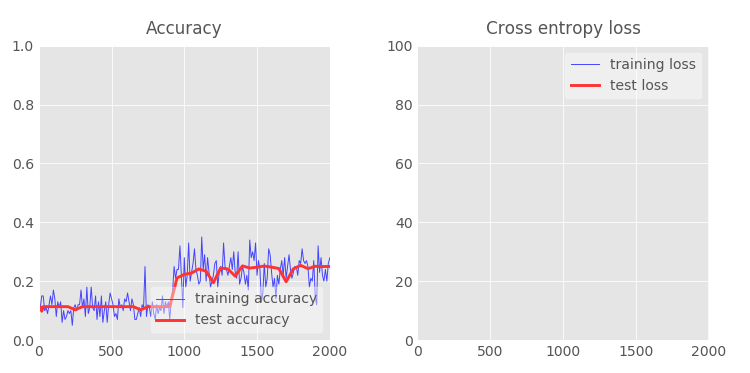
\includegraphics[width=6cm]{Images/MNIST_CNN_S1E3.png}}
\caption{\label{fig:MNIST_CNN_S1E3} The performance of convolutional neural network model using Softmax.}
\end{figure}
\\Result: the performance of this model is shown in Figure~\ref{fig:MNIST_CNN_S1E3}. The accuracy is just 0.2538, and the loss is 176.525. The loss is too high so its curve is disappeared in this figure. The performance of this model is too bad, so that Softmax is excluded.
%
\subsubsection{Experiment 4: using Tanh}
In this experiment, Tanh is used as activation function.
\begin{figure}[h]
\centering
\fboxsep 2mm
\framebox{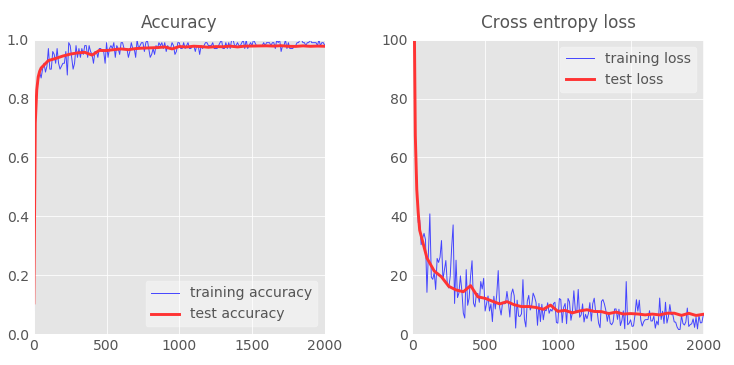
\includegraphics[width=6cm]{Images/MNIST_CNN_S1E4.png}}
\caption{\label{fig:MNIST_CNN_S1E4} The performance of convolutional neural network model using Tanh.}
\end{figure}
\\Result: the performance of this model is shown in Figure~\ref{fig:MNIST_CNN_S1E4}. The accuracy is 0.9797, and the loss is 6.51466. The performance of this model is better than using Sigmoid, but worse than using ReLU.
%
\subsubsection{Experiment 5: using Softplus}
In this experiment, Softplus is used as activation function.
\begin{figure}[h]
\centering
\fboxsep 2mm
\framebox{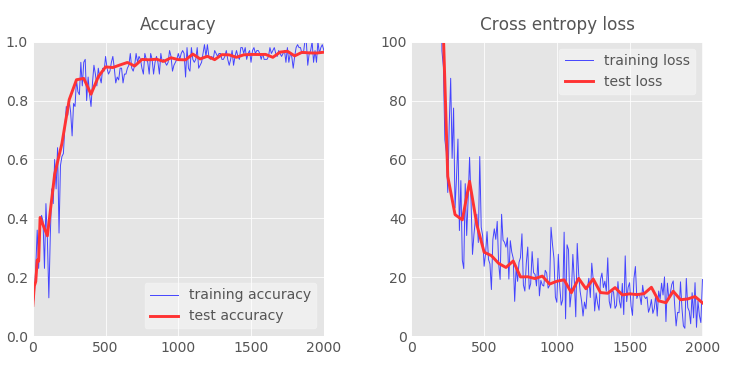
\includegraphics[width=6cm]{Images/MNIST_CNN_S1E5.png}}
\caption{\label{fig:MNIST_CNN_S1E5} The performance of convolutional neural network model using Softplus.}
\end{figure}
\\Result: the performance of this model is shown in Figure~\ref{fig:MNIST_CNN_S1E5}. The accuracy is 0.9676, and the test loss is 11.3303. The performance of this model is not as good as the model using Tanh and ReLU. According to figure, the fluctuation of the accuracy and loss is quite notable.
%
\subsubsection{Experiment 6: using ELU}
In this experiment, change the activation function to ELU.
\begin{figure}[h]
\centering
\fboxsep 2mm
\framebox{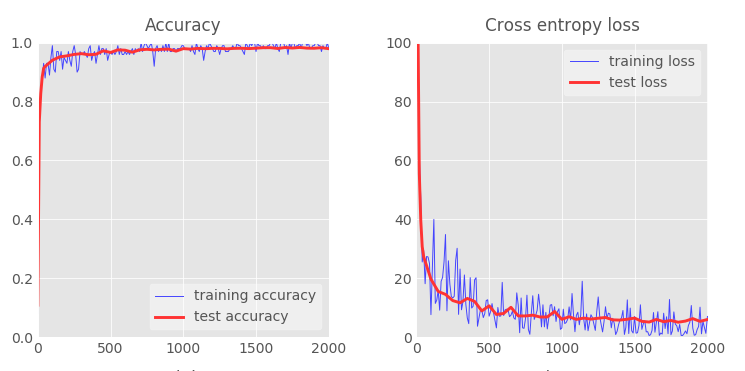
\includegraphics[width=6cm]{Images/MNIST_CNN_S1E6.png}}
\caption{\label{fig:MNIST_CNN_S1E6} The performance of convolutional neural network model using ELU.}
\end{figure}
\\Result: the performance of this model is shown in Figure~\ref{fig:MNIST_CNN_S1E6}. The accuracy is 0.9839, and the test loss is 5.03941. The performance of this model is better than all of the pervious models. 
\subsubsection{Summary}
According to the result of these six experiments, ReLU and ELU are more suitable than other four functions for this image classification task. Because the model using ELU get the best result in experiment, the following experiments will use ELU as activation Function in convolutional layer and dense layer.
%
\subsection{Scenario 2: Changing the Pooling Function of Pooling Layer}
Polling function in pooling layer can reduce the dimensionality of the features and extract the important information to improve the performance of the convolutional neural network model. Average pooling and Max polling are two common functions in polling layer.

Because the Max pooling has been used in previous experiments, in this Scenario, based on the model in Experiment 6 Scenario 1, we changed the pooling function to average polling. Other features of the neural network remain unchanged.

Other features of the neural network in this scenario:
\begin{itemize}
\item {\sl Number of layers: } 4
\item {\sl Activation Function in logits layer:} Softmax
\item {\sl Activation Function in convolutional layer and dense layer} ELU
\item {\sl Loss Function:} cross-entropy
\item {\sl Learning Rate: } 0.003
\end{itemize}
\begin{figure}[h]
\centering
\fboxsep 2mm
\framebox{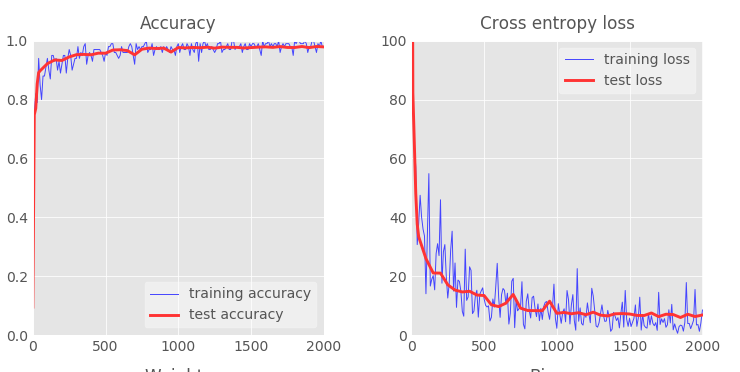
\includegraphics[width=6cm]{Images/MNIST_CNN_S2E1.png}}
\caption{\label{fig:MNIST_CNN_S2E1} The performance of convolutional neural network model using Average Pooling.}
\end{figure}
Result: The result of this experiment is shown in Figure~\ref{fig:MNIST_CNN_S2E1} above. The accuracy is 0.9803 and the loss is 5.96717. The performance of this model is lower than the model using Max pooling, whose accuracy is 0.9839. So the Max pooling function will still be used in pooling layer in following experiments.
%
\subsection{Scenario 3: Implement Learning Rate Decay}
Observing the plots of previse experiment, the fluctuation of accuracy and loss is significant. To reduce this noise, the technique of learning rate decay is a good approach. 

In this experiment, based on the convolutional neural network model we established in Experiment 6 Scenario 1, learning rate decay is implemented to improve the performance of the model. The learning rate decays from 0.003 to 0.0001 during this experiment and other configuration remain unchanged.
\begin{figure}[h]
\centering
\fboxsep 2mm
\framebox{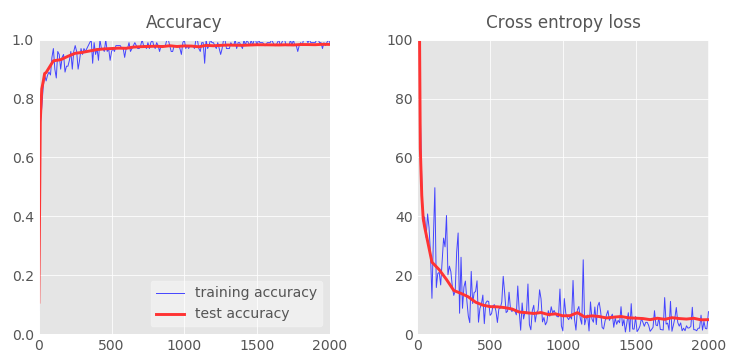
\includegraphics[width=6cm]{Images/MNIST_CNN_S3E1.png}}
\caption{\label{fig:MNIST_CNN_S3E1} The performance of the convolutional neural network implemented learning rate decay.}
\end{figure}
\\Result: The result of this experiment is shown in Figure~\ref{fig:MNIST_CNN_S3E1} above. The accuracy is 0.9843 and the loss is 4.8379. The performance is slight improved comparing with the model without implementing learning rate decay, whose accuracy is 0.9839, and the noise of the curves is reduced too. So this useful technique will be used in following experiments.
%
\subsection{Scenario 4: Adding more layers into Convolutional Neural Network model}
In neural network, more layers usually means more trainable weights and biases, means the increase of the degrees of freedom. In this scenario, based on the CNN model in Scenario 3, add one convolutional layer and one pooling layer into the model. The architecture of this model is shown in Figure~\ref{fig:MNIST_CNN_S4_Architecture} below.
\begin{figure}[h]
\centering
\fboxsep 2mm
\framebox{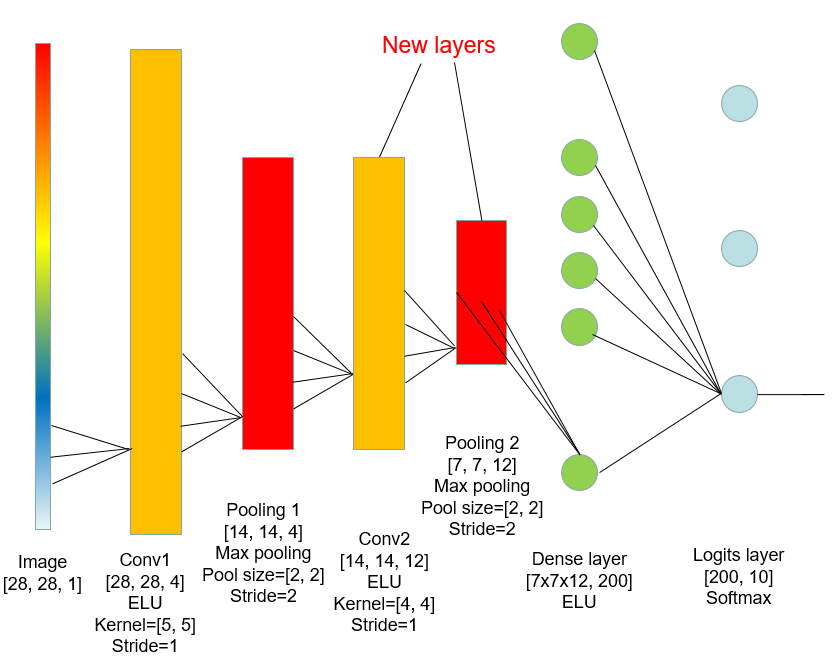
\includegraphics[width=6cm]{Images/MNIST_CNN_S4_Architecture.png}}
\caption{\label{fig:MNIST_CNN_S4_Architecture} The architecture of the CNN model in this Scenario.}
\end{figure}
\subsubsection{Experiment 1}
Result: The result of this experiment is shown in Figure~\ref{fig:MNIST_CNN_S4E1}. The accuracy is 0.9899 and the test loss is 3.16573. The performance of this model is better than the one in scenario 3, whose accuracy is 0.9843. It clearly shows that add more layer is a useful way to optimize the model.
\begin{figure}[h]
\centering
\fboxsep 2mm
\framebox{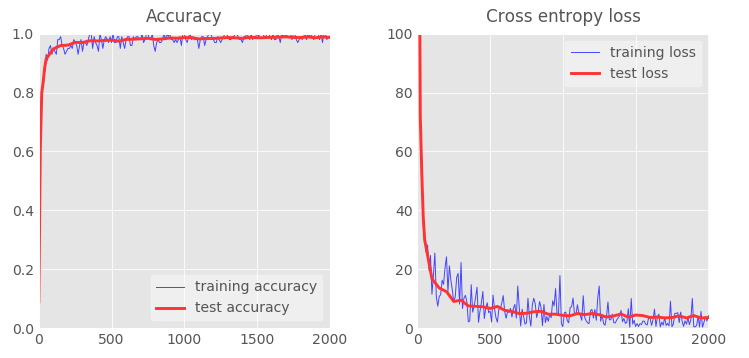
\includegraphics[width=6cm]{Images/MNIST_CNN_S4E1.png}}
\caption{\label{fig:MNIST_CNN_S4E1} The performance of the model with two convolutional layers and two pooling layers.}
\end{figure}
\subsubsection{Experiment 2}
Because of the limitation of the computer’s capability, in previous experiments the training process just lasted 4 epochs (2400 steps). Now expand the training process to 20 epochs (12000 steps) in this experiment to test the performance of the model. The result is shown in Figure~\ref{fig:MNIST_CNN_S4E2}. The accuracy increased 0.9914, and the loss is 3.86256.
\begin{figure}[h]
\centering
\fboxsep 2mm
\framebox{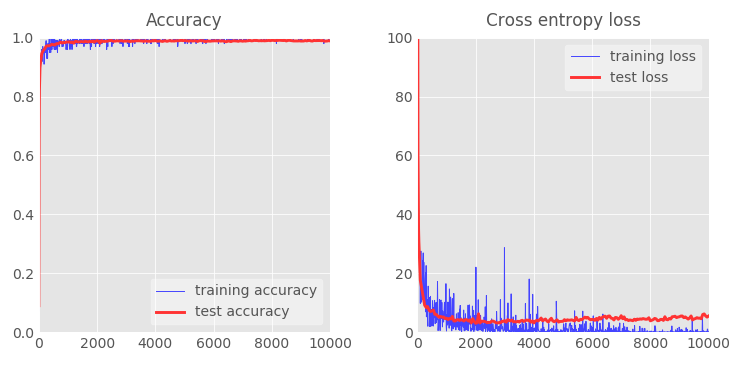
\includegraphics[width=6cm]{Images/MNIST_CNN_S4E2.png}}
\caption{\label{fig:MNIST_CNN_S4E2} The same model but lasts 20 epochs.}
\end{figure}
%
\subsection{Scenario 5: Implement neuron dropout to avoid overfitting}
According to the plots of the  Experiment 2 in last scenario (as shown in Figure~\ref{fig:MNIST_CNN_S4E2}), the test loss slightly increases when the training loss continuously decreases. This phenomenon is what we called "overfitting". To avoid overfitting problem, the neuron dropout is a useful approach, which will randomly drop some neurons from neural network during training process. 

The CNN model in this scenario is based on the model in Experiment 2 Scenario 4. The dropout mechanism is implemented in dense layer, and 25\% of neurons are dropped in this layer.  
\begin{figure}[h]
\centering
\fboxsep 2mm
\framebox{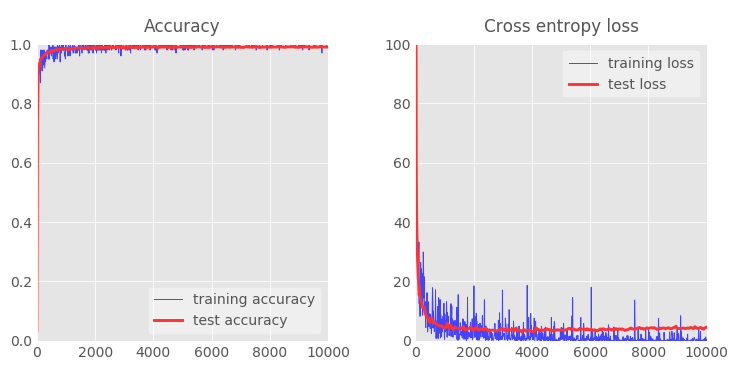
\includegraphics[width=6cm]{Images/MNIST_CNN_S5E1.png}}
\caption{\label{fig:MNIST_CNN_S5E1} The performance of the CNN model implemented dropout.}
\end{figure}
Result: The result of this experiment is shown in Figure~\ref{fig:MNIST_CNN_S5E1} above. The accuracy is 0.9917, and the loss is 2.96396. The performance have slightly improved by implement dropout mechanism and the overfitting problem is relieved according to these plot

This is the best CNN model build in this project for the classification of MNIST dataset.
%%%%%%%%%%%%%%%%%%%%%%
%%% The Classification of  CIFAR-10 colour images
\chapter{\label{chapter4}The Classification of CIFAR-10 colour images}
\section{Introduction}
The CIFAR-10 dataset contains 60,000 colour images of 10 different classes, and the size of these images is 32*32. 50,000 images are used for training the neural network and 10,000 images are for test. Because these images have more pixels and the shape of the objects inside these images are more complicated, it is much more different to classify these images than handwritten digits images. The CIFAR-10 dataset used in this project is come from the source\footnote{\url{https://www.cs.toronto.edu/~kriz/cifar-100-python.tar.gz}.}.

To achieve the goal of successfully classifying these images, at first, a benchmark is chosen from the state-of-the-art approaches~\cite{Lars:2015}, and the convolutional neural network model of the benchmark is reproduced based on the paper. After that, based on the best CNN model that we established for the classification of MNIST handwritten digital images, we improve that model to catch the benchmark. In this process, the original CNN model is adjusted by changing the functions and architecture of the neural network, or implementing some useful mechanisms. 

Since the images in CIFAR-10 database are more complicated than MNIST database, to better learn the information contained in each images, each experiment lasts 30 epochs. Each epoch contains 500 training iterations and 5 test iterations. The batch size of both training and test iterations are 100.
\subsection{Technique}
The codes are written in Python, and TensorFlow is used.
\subsection{Experiment Environment}
Because the training of CNN model involves huge amount of computing workload, to accelerate the raining process, the training work is moved  to a server from laptop.
\begin{itemize}
\item {\sl Processor:} Intel(R) Xeon(R) CPU E5-2695 v4 @ 2.10GHz.
\item {\sl Mem:} 504 GB.
\item {\sl OS:} Ubuntu 16.04.4 LTS.
\end{itemize}
%  Benchmark
\section{Benchmark}
The performance benchmark for classifying CIFAR-10 database with CNN is reproduced from the paper titled \emph{Deep Convolutional Neural Networks as Generic Feature Extractors}~\cite{Lars:2015}. This paper is come from the source\footnote{\url{http://www.isip.uni-luebeck.de/fileadmin/uploads/tx_wapublications/hertel_ijcnn_2015.pdf}.}.

The CNN model in this paper contains 24 layers in total, including five convolutional layers, three maximum pooling layers and three fully connected layers. The architecture of the convolutional neural network model in paper is show in Figure~\ref{fig:The_Architecture_of_Benchmark_model}. This model implemented both weight decay and learning rete decay. The parameter of weight decay is 0.00005 and the learning rate decreases from 0.001 to 0.00001 in first 20 epochs. To avoid overfitting problem, this model also implemented batch normalization and neuron dropout. To get the best result, they trained the model for 30 epochs and in each iteration, and the batch size is 80. 
\begin{figure}[h]
\centering
\fboxsep 2mm
\framebox{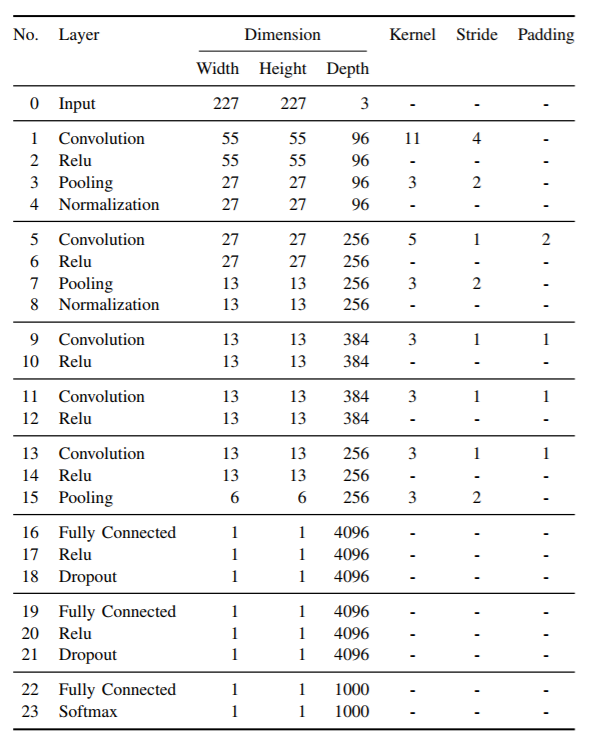
\includegraphics[width=6cm]{Images/The_Architecture_of_Benchmark_model.png}}
\caption{\label{fig:The_Architecture_of_Benchmark_model} The architecture of the benchmark CNN model.}
\end{figure}
\\We reproduced this convolution neural network model and got a accuracy of 79.6\%. The result of this experiment is shown in Figure~\ref{fig:The_performance_of_Benchmark} below. However, this result is far away from the best result in paper, which is 89.99\%. This difference is mainly caused by three reasons. 

One reason is that they trained the CNN model on a huge database before trained on CIFAR-10, but we did not. According to the paper, they divided this CNN model into two parts, feature extraction part and classification part(fully-connected layers). They trained the CNN model with the ILSVRC-12 dataset first, which contains nearly 1.5 million colour images for 1,000 different categories. After that, they maintained the feature extraction part and retrained the classification part on different datasets, including CIFAR-10. That model achieved an accuracy of 89.14\% on CIFAR-10 dataset. In last step, they retrained entire convolutional neural network on CIFAR-10 database and achieved an accuracy of 89.99\%. Since we did not have enough time and resource to carry out this kind of pre-training work, the performance of reproduction is not as good as the paper described.

Another reason for the difference is that they resized the images from 32*32 to 272*272 and increased the training set by cropping each resized image several times (corners  and center) before feeding them into the neural network.

The last possible reason for the bad performance is that we changed the number of neurons in each layer in experiment, and that reduced the amount of information that can be preserve in neural network. Because the lack of training on ILSVRC-12 dataset, when the images are resized to 227*227 and feed them into the model, the neural network failed to learn the features. Therefore, to achieve the goal of classifying these images, we shrink the size of the each layer.
\begin{figure}[h]
\centering
\fboxsep 2mm
\framebox{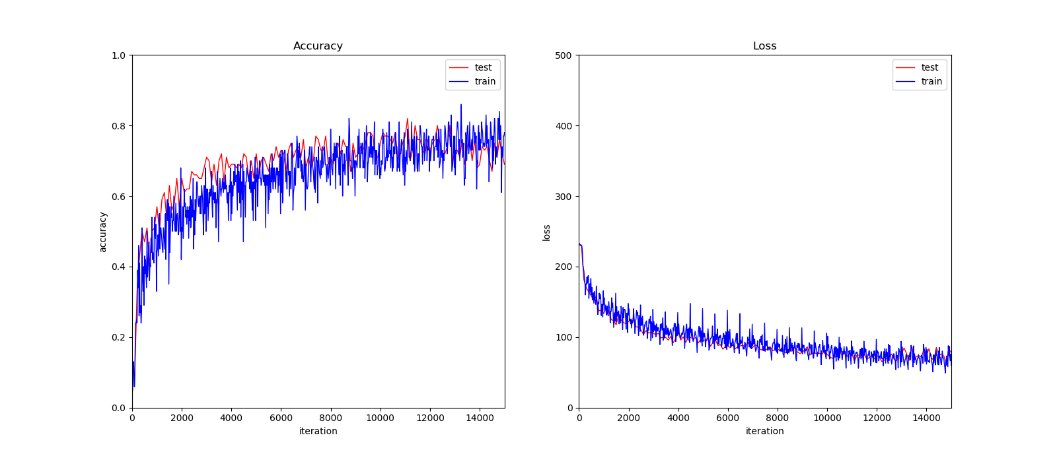
\includegraphics[width=6cm]{Images/The_performance_of_Benchmark.png}}
\caption{\label{fig:The_performance_of_Benchmark} The performance of the reproduced CNN model.}
\end{figure}
%%% Develop a CNN model
\section{Building a CNN model for classifying CIFAR-10 images}
This section will introduce the process of building and training a suitable CNN model for classifying CIFAR-10 colour images. Since we have built a good CNN model for MNIST database, the CNN model for CIFAR-10 will begin from that model. Then, changing the model by using different activation function, adding more layers or implementing some useful techniques in model. The experiments in this section lasts 30 epochs and the batch size is 100. 

Because the CNN model for classifying CIFAR-10 images is much more complicated than the models for MNIST database, the development process become complicated too. Here are the basic rules we followed in development process:
\begin{itemize}
\item Make sure in each experiment only one of the neural network’s features is changed. Keep the change if it does improve the performance of CNN model. 
\item Always try to add more layers into the model if they does not undermined the performance, because more layers always means more trainable parameters, means more information can be stored in neural network.
\item If the result of experiment shows that there are some problems in model, for example the overfitting problem, try to solve it first, before changing the next key feature.
\end{itemize}
%%
\subsection{Scenario 1: Using the best CNN model build for classifying MNIST images to classify CIFAR-10 images}
Through the experiments of classifying the MNIST images before, we got a nice convolutional neural network model. In this scenario, we applied this model in classifying the CIFAR-10 images. This model consists of 12 layers. The architecture of this CNN model is shown in Figure ~\ref{fig:CIFAR_10_CNN_S1_Architecture}
\begin{figure}[h]
\centering
\fboxsep 2mm
\framebox{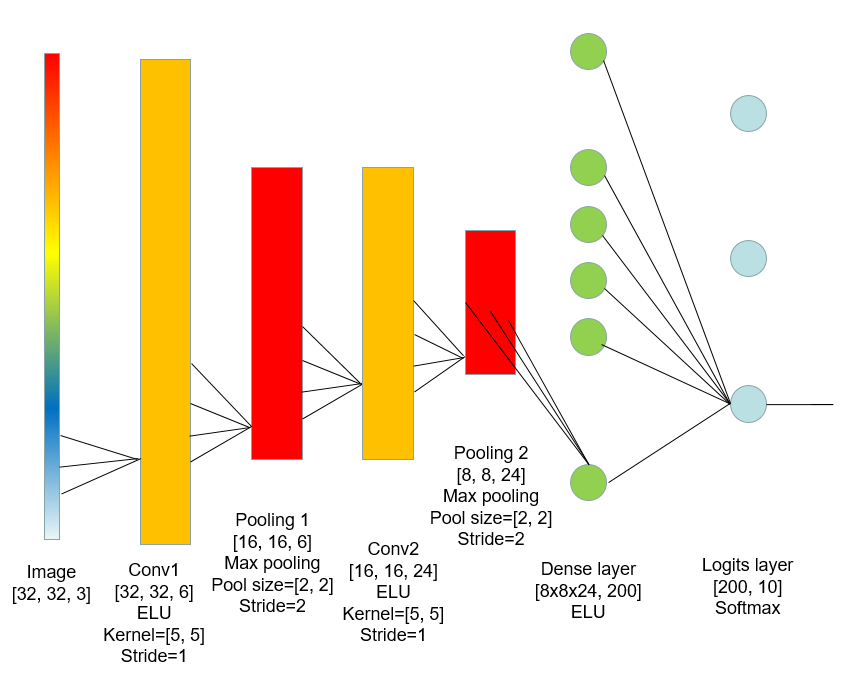
\includegraphics[width=6cm]{Images/CIFAR_10_CNN_S1_Architecture.png}}
\caption{\label{fig:CIFAR_10_CNN_S1_Architecture} The architecture of the benchmark CNN model.}
\end{figure}
\\Important features of this CNN model:
\begin{itemize}
\item {\sl Number of layers:} 4
\item {\sl Activation Function in logits layer:} Softmax
\item {\sl Activation Function in convolutional layer and dense layer} ELU
\item {\sl Loss Function:} cross-entropy
\item {\sl Learning Rate:} decays from 0.003 to 0.00001
\item {\sl Dropout rate: 0.25}
\end{itemize}
Result: The result of this experiment is shown in Figure~\ref{fig:CIFAR_10_CNN_S1E1} below. The accuracy is 0.656 and the loss is 83.382. The performance of this model is lower than the benchmark. In addition, according the curve of test loss, this model have a serious overfitting problem. The test loss continually increases while the test loss decreases after about 2000 iterations (4 epochs). In following experiment, we tried to solve this problem and improve the performance.
\begin{figure}[h]
\centering
\fboxsep 2mm
\framebox{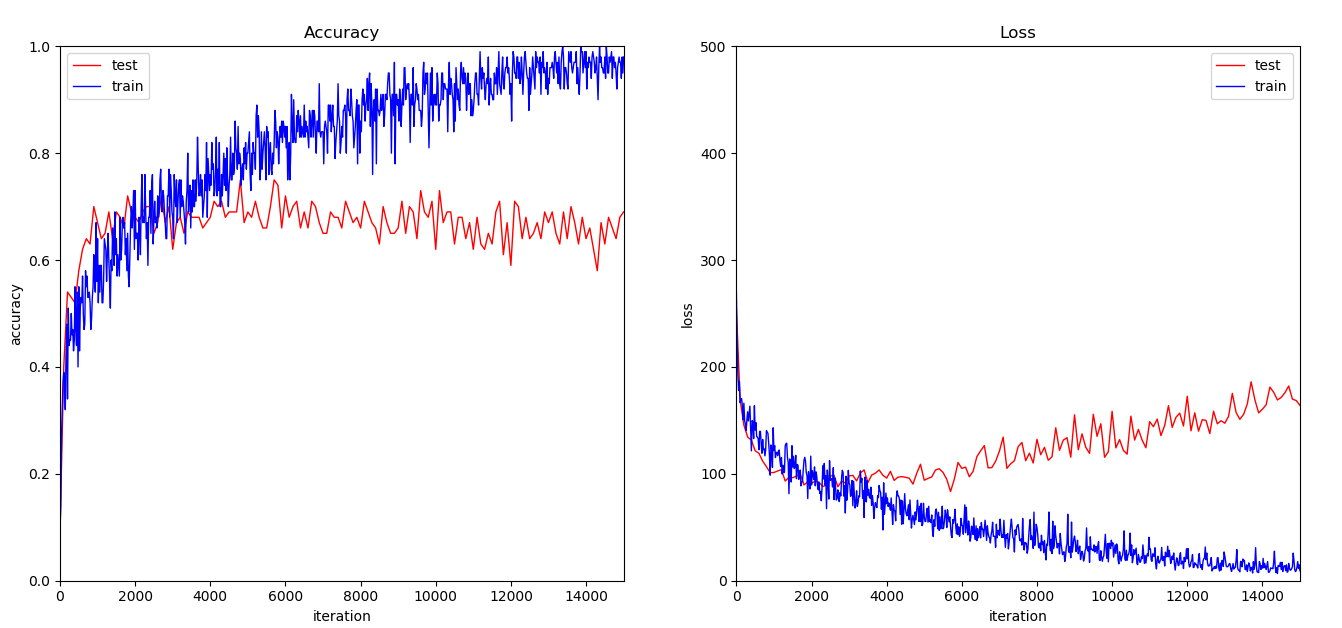
\includegraphics[width=6cm]{Images/CIFAR_10_CNN_S1E1.png}}
\caption{\label{fig:CIFAR_10_CNN_S1E1} The performance of the best model established for MNIST database classifying CIFAR-10 images.}
\end{figure}
%%
\subsection{Scenario 2: Implementing dropout in every convolutional layers to relieve the overfitting problem}
In last scenario, only the dense layer have implemented the neuron dropout mechanism. To solve the overfitting problem, in this experiment, dropout will be implemented in every convolutional layers. Other features of the model remain unchanged
\begin{figure}[h]
\centering
\fboxsep 2mm
\framebox{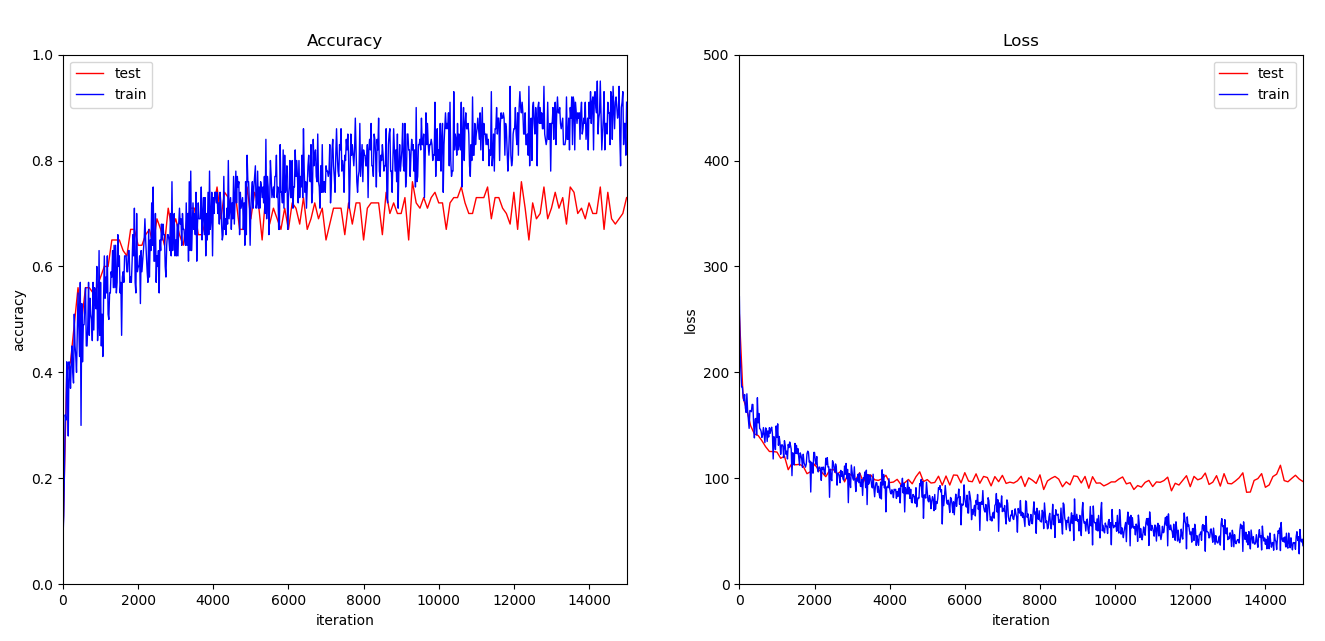
\includegraphics[width=6cm]{Images/CIFAR_10_CNN_S2E1.png}}
\caption{\label{fig:CIFAR_10_CNN_S2E1} The performance of the CNN model with dropout in every convolutional layers.}
\end{figure}
\\Result: The result of this experiment shown in Figure~\ref{fig:CIFAR_10_CNN_S2E1}. The accuracy dramatically increased from 0.656 to 0.71. Meanwhile, according to the loss curves in plot, the test loss does not increase this time, which means the overfitting problem is relieved. Therefore, to avoid overfitting, this neuron dropout will be implemented in every convolutional layers in following experiments. 
%%
\subsection{Scenario 3: Adding more convolutional layers into the model}
In convolutional neural network, pooling layer is always used in conjunction with convolutional layers. In this experiment, for better understanding, the pooling layer and the convolutional layers before it are viewed as a unit, as a convolutional module. Therefore there are two convolutional modules exist in the CNN mode in last scenario. 

Because the images in CIFAR-10 dataset are more complicated than the handwritten digits images in MNIST, to better extract the information inside these images, in this scenario, more convolutional layers were added before each convolutional module. 
%
\subsubsection{Experiment 1 and 2}
Based on the CNN model in Scenario 2, we successively added two new convolutional layers into the model before the first convolutional module in experiment 1 and experiment 2.
Result: In experiment 1, with one layer added, the accuracy decreased to 0.70. With two layers added in experiment 2, the maximum accuracy notably increased to 0.8, and the average is 0.6984. The experiment result of the model with two added is shown in Figure ~\ref{fig:CIFAR_10_CNN_S3E2}. 
\begin{figure}[h]
\centering
\fboxsep 2mm
\framebox{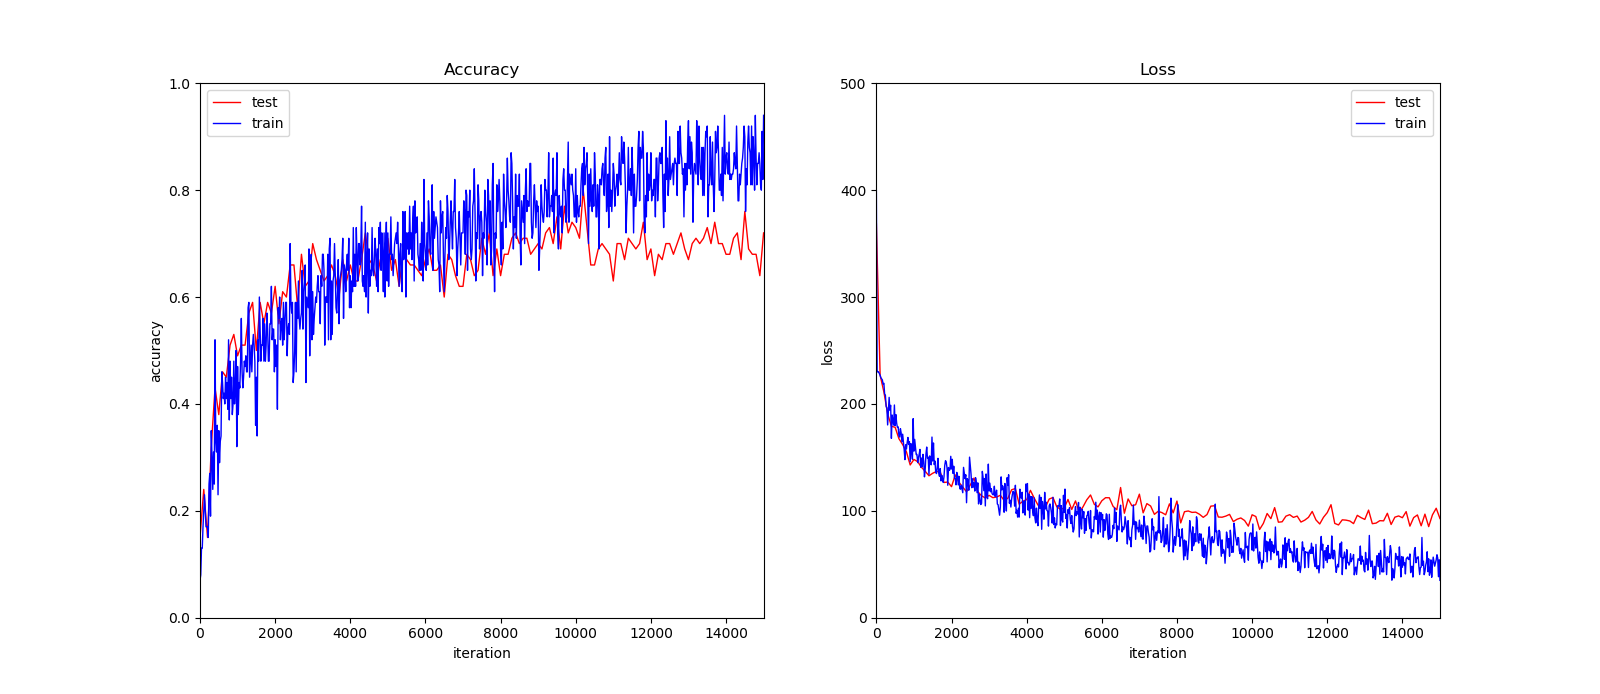
\includegraphics[width=6cm]{Images/CIFAR_10_CNN_S3E2.png}}
\caption{\label{fig:CIFAR_10_CNN_S3E2} The performance of the CNN model with two new convolutional layers added before the first convolutional module.}
\end{figure}
%
\subsubsection{Experiment 3 and 4}
Based on the CNN model in Experiment 2, we successively added two other new convolutional layers into the model before the second convolutional module in experiment 3 and experiment 4.

Result: With one new layer added in experiment 3, the accuracy decrease to 0.6692 and the loss increases to 91.560295. With two layers added in experiment 4, the performance even become worse. The accuracy is only 0.6352 and the loss grows to 98.860596. Clearly, these two layers undermined the performance. Therefore, these two layers are temporarily abandoned.  The neural network is rolled back to the model in experiment 2. The performance of the model with two new layers added in experiment 4 is shown in Figure~\ref{fig:CIFAR_10_CNN_S3E4}.
\begin{figure}[h]
\centering
\fboxsep 2mm
\framebox{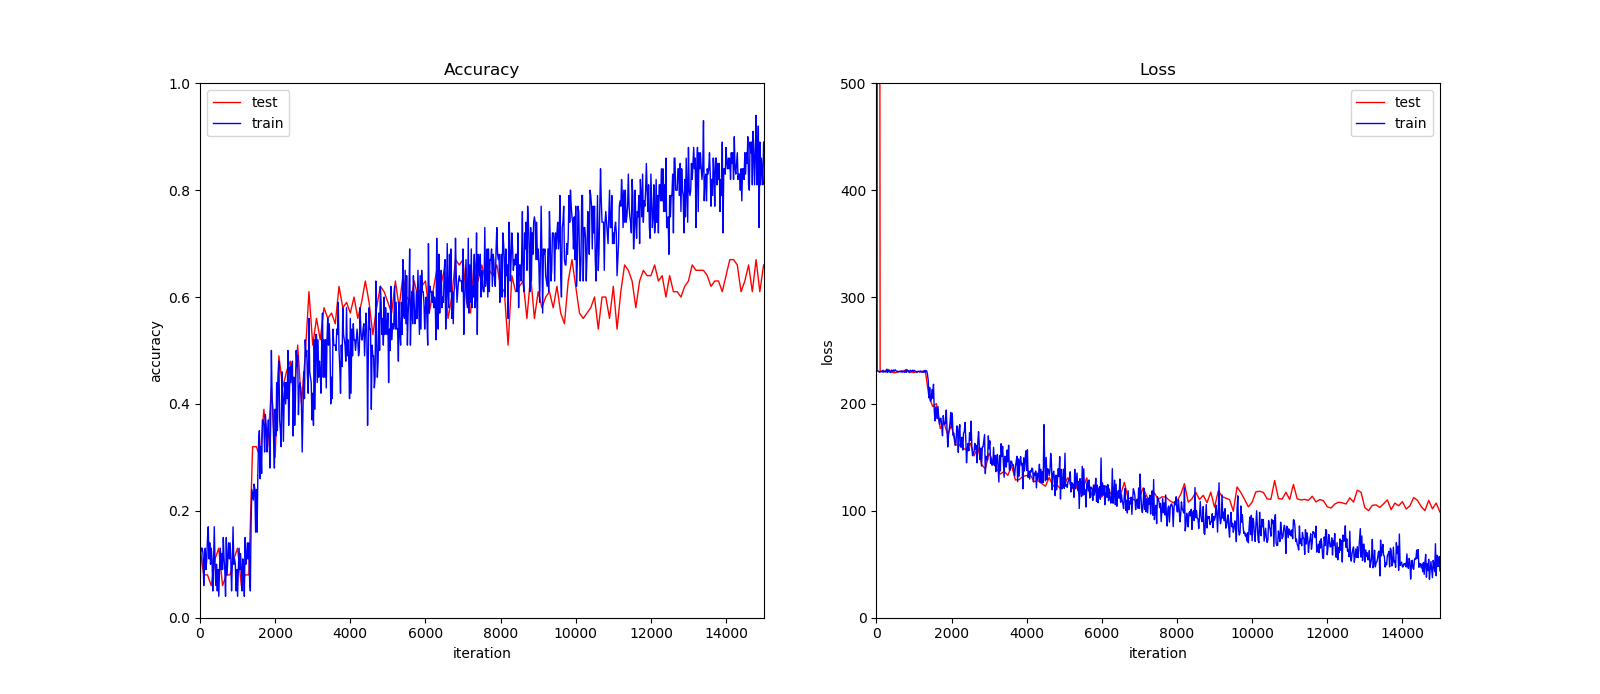
\includegraphics[width=6cm]{Images/CIFAR_10_CNN_S3E4.png}}
\caption{\label{fig:CIFAR_10_CNN_S3E4} The performance of the CNN model with two new convolutional layers added before the second convolutional module.}
\end{figure}
%%
\subsection{Scenario 4: Adding one more convolutional module}
Because the size of images in CIFAR-10 database is 32*32, which are bigger than 28*28 hand written digital images in MNIST database, and the stride of pooling is 2, we can added one more convolutional module into the model in Experiment 2 Scenario 3 before the dense layer. The activation function in new convolutional layer is ReLU and the pooling function in new polling layer is Max Polling.
\begin{figure}[h]
\centering
\fboxsep 2mm
\framebox{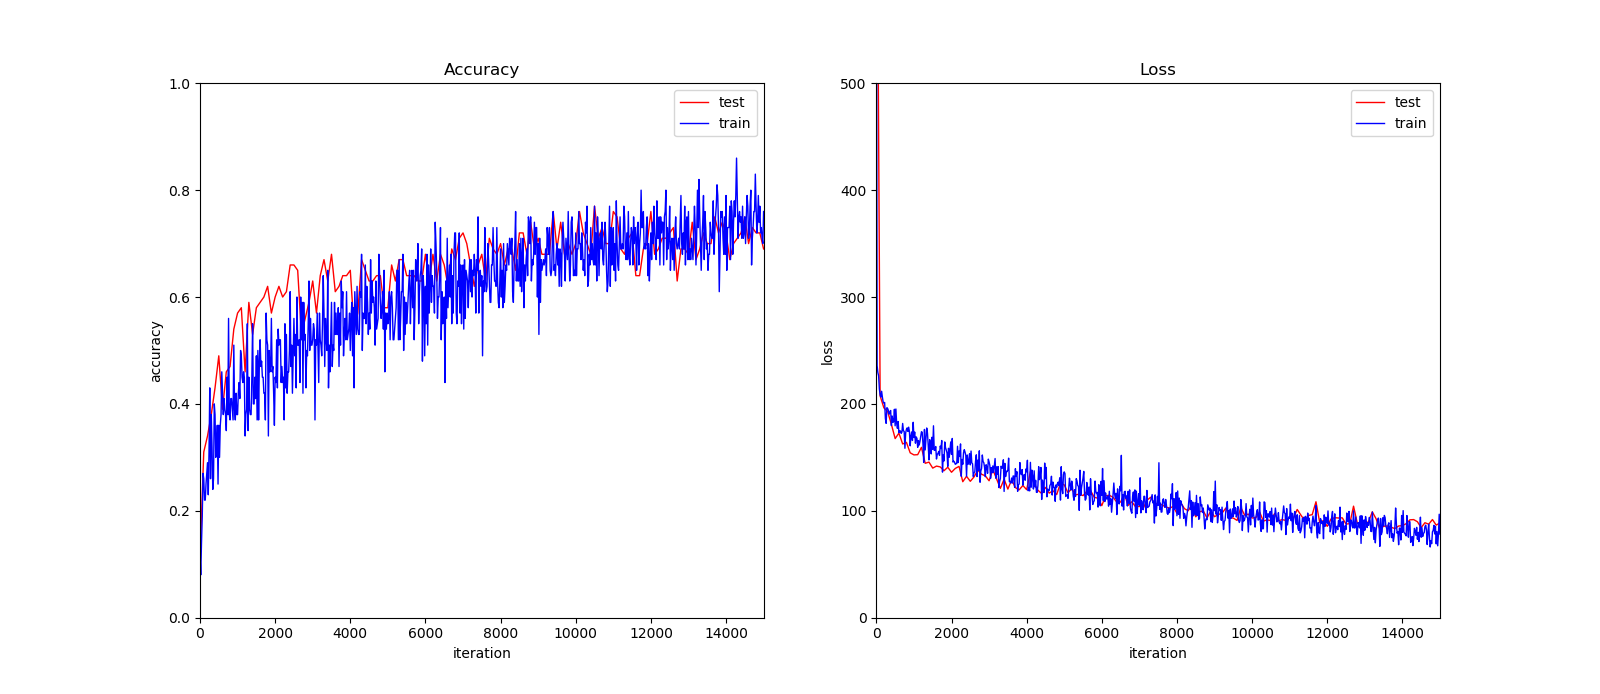
\includegraphics[width=6cm]{Images/CIFAR_10_CNN_S4E1.png}}
\caption{\label{fig:CIFAR_10_CNN_S4E1} The performance of the CNN model with new convolutional module added.}
\end{figure}
\\Result: The result of this experiment is shown in Figure~\ref{fig:CIFAR_10_CNN_S4E1}. The accuracy is 0.7084 and the loss is 82.74115. Although the performance of this model did not improve a lot compared with the result in Experiment 2 Scenario 3, we still prefer to keep these two new layers since the training and the test results of this model are more closer, and the overfitting problem is completely disappeared in this model.
%%
\subsection{Scenario 5: Adding Normalization Layers into the model}
Batch normalization is a useful technique in neural network. It can speeds up the training process and makes each layer of a neural network more independent. In this scenario, we implemented this technique to each convolutional module by adding a normalization layer after each pooling layer. Because there are three convolutional modules in the CNN model in last experiment, we added three normalization layers successively into this model. 
%
\subsubsection{Experiment 1: Adding a normalization layer after the first convolutional module}
Based on the CNN model in last scenario, in this experiment, we added one normalization layer after the first convolutional module.

Result: With one normalization layer added, the accuracy slightly increased to 0.7176 and the loss decreased to 74.17486.
%
\subsubsection{Experiment 2: Adding a normalization layer after the second convolutional module}
In this experiment, we added one more normalization layer in to the model after the second convolutional module.

Result: With two normalization layers added, the accuracy increased to 0.7592 and the loss declined to 70.14456.

However, when we run the program second time, the neural network failed to classify the images. The accuracy is just about 10\% and the loss is around 230. After several experiments, we realized sometimes it works and sometimes not. Since this problem may caused by the dead ReLU problem, which will result in that some of the neurons will never be activated and the training of parameters fail. To fix this problem, the Exponential Linear Units (ELU) function is used to replace the ReLU in next experiments.
%
\subsubsection{Experiment 3: Replace the ReLU with ELU}
In this experiment, ReLU is replaced by ELU in convolutional layers and dense layer (the fully-connected layer before output layer).

Result: With the same model but using different activation function, ELU, the accuracy dramatically increased to 0.8096 and the loss declined to 61.542137. Meanwhile, the performance of this CNN model is more stable in repeated experiments. Obviously, the performance improved a lot with ELU, so the ELU was used in following experiments.
%
\subsubsection{Experiment 4: Adding a normalization layer after the last convolutional module}
In this experiment, we added one more normalization layer in to the model after the last convolutional module. 

Result: The accuracy is 0.8104 and the loss decreased to 52.059204. The result of this experiment is shown in Figure~\ref{fig:CIFAR_10_CNN_S5E4}.
\begin{figure}[h]
\centering
\fboxsep 2mm
\framebox{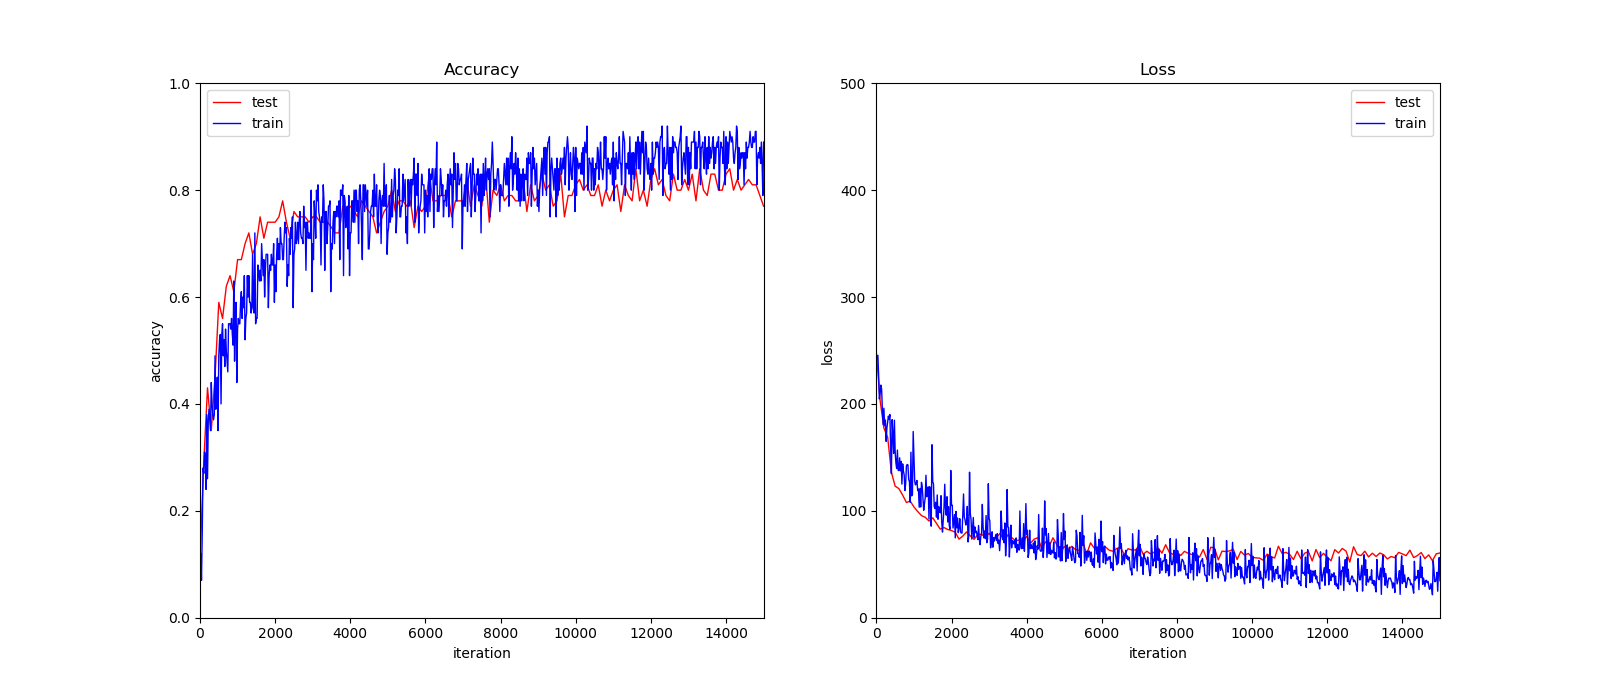
\includegraphics[width=6cm]{Images/CIFAR_10_CNN_S5E4.png}}
\caption{\label{fig:CIFAR_10_CNN_S5E4} The performance of the CNN model with three new normalization layers added.}
\end{figure}
%%
\subsection{Scenario 6: Adding more convolutional layers before last two convolutional modules}
To increase the depth of the neural network and its ability of extracting features, in this scenario, we added two new convolutional layers before the second and third convolutional module respectively. Actually, we tried to add more convolutions, but the training of the model is failed in those experiments. Therefore, those experiments are omitted in this report. The model in this scenario is based on the model established in Experiment 4 Scenario 5.

Result: With two new convolutional layers added before the second convolutional module and the third convolutional module respectively, the accuracy increased to 0.8464 and the loss decreased to 52.166866. The performance of this model is better than the benchmark. To be specific, the result is better than the benchmark model reproduced from that paper, but is not as good as the best result described in paper. The result of this experiment is shown in Figure~\ref{fig:CIFAR_10_CNN_S6E1}.
\begin{figure}[h]
\centering
\fboxsep 2mm
\framebox{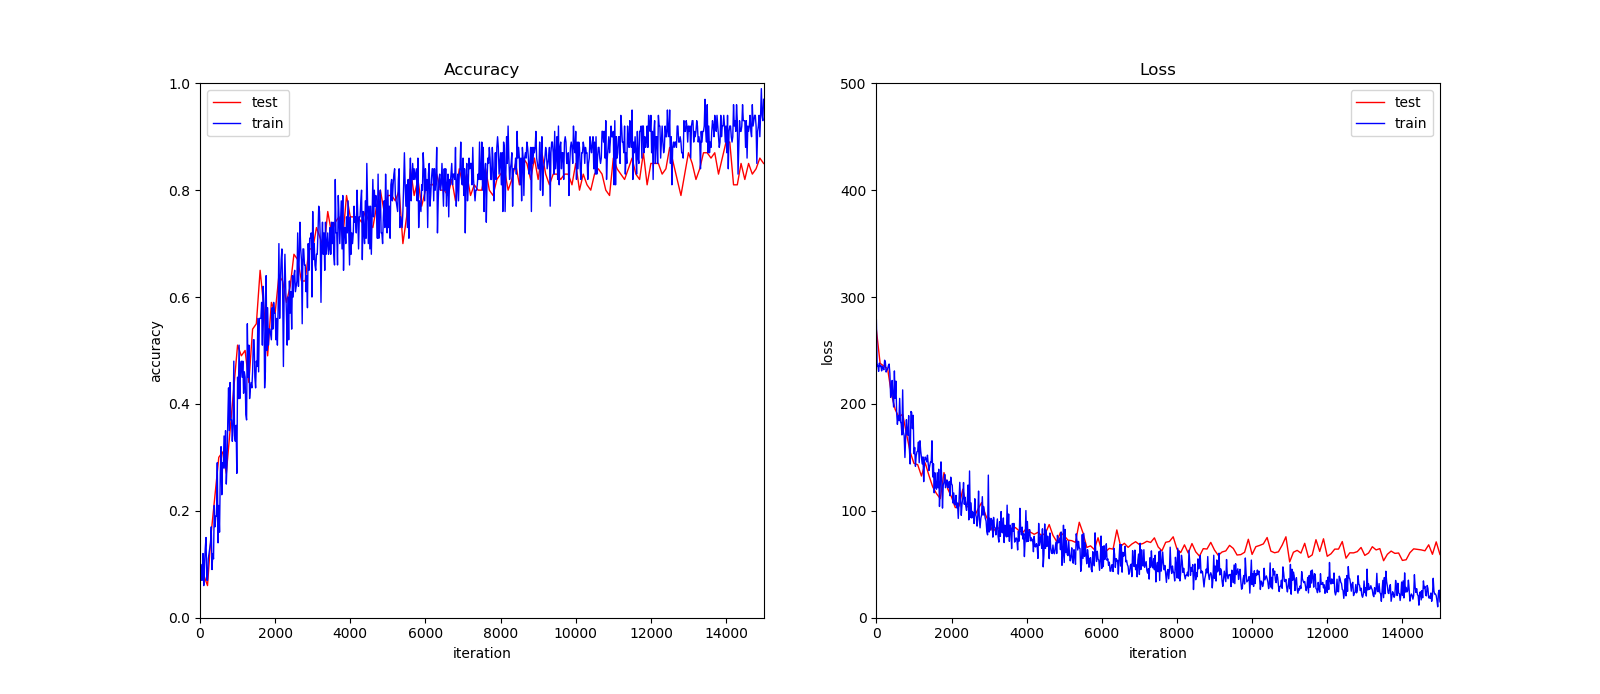
\includegraphics[width=6cm]{Images/CIFAR_10_CNN_S6E1.png}}
\caption{\label{fig:CIFAR_10_CNN_S6E1} The performance of the CNN model with three new normalization layers added.}
\end{figure}
\\The CNN model in this experiment is the best model we build for classifying CIFAR-10 color images. The full architecture of this model is shown in Figure~\ref{fig:Full_Architecture_of_CNN} below.
\begin{figure}[h]
\centering
\fboxsep 2mm
\framebox{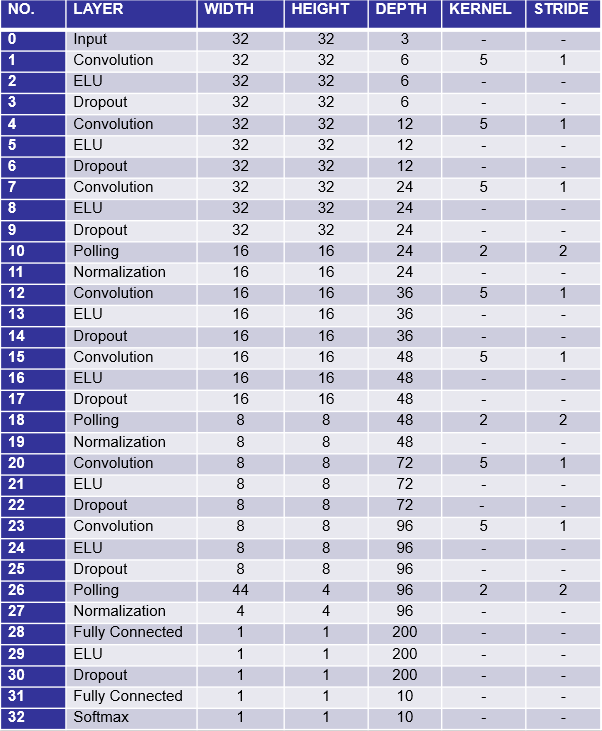
\includegraphics[width=6cm]{Images/Full_Architecture_of_CNN.png}}
\caption{\label{fig:Full_Architecture_of_CNN} The full achitecture of the CNN model developed for classifying CIFAR-10 images.}
\end{figure}
%%%%%%%%%%%%%%%%%%%%%%%  Chapter 5 %%%%%%%%%%%%%%%%%%%%%%%%%
\chapter{\label{chapter5}Implementation and Evaluation}
The objective of this project is the design and implementation of deep neural networks in different classification problems. The experiments in this project have been written in python and using Tensorflow.
Since the core object of this project is to develop and train neural networks for classifying images, the implementation of neural networks is one of the most important tasks that throughout the project. The programs developed in each of the experiments in this project are written in python, and the neural network models are built in TensorFlow. 

The experiments in this project mainly consists of three parts: 
\begin{enumerate}
\item {\sl Design a neural network model:} The architecture of the network is designed selecting the number of neurons, convolutional layers, dense layers, regularization, loss function, activation functions, etc. 
\item {\sl Data preparation:} In this part, images and labels are loaded and they are processed to the format for feeding into the neural network.
\item {\sl Training the model:} The training process is defined, including the batch size and total epochs, learning rate (if implemented learning rate decay)
\end{enumerate}

In this project, the models are evaluated with the loss and accuracy every 100 batches. The global  performance is measured by the average accuracy and loss on the test set. However, because in the early stages of this project, only maximum accuracy and minimum loss were recorded in training process, the accuracy and loss used to evaluate the global performance are not average value in these experiments. This is a weakness of this project. Although the experiments involve CIFAR-10 dataset have been redid and the changes made in development process have been reevaluated, we did not have enough time to redo the experiments on MNIST dataset.

As mentioned above, both MNIST database and CIFAR-10 database are split into training and test set. In each experiment, the neural network model is tested during the training process by feeding the test data into the model after every 100 batches. The accuracy and loss of the test iterations (batches) and part of the training iterations are recorded for demonstrating the performance in plots and calculating the average performance.
%%%%%%%%%%%%%%%%%%%%%%%  Chapter 6 %%%%%%%%%%%%%%%%%%%%%%%%%
\chapter{\label{chapter6}Conclusions and Future Work}
This project focuses on the development of deep neural network for image classification. In the first part of this project, a background research on the principle of neural network has been done. After that, these concepts have been applied in solving an initial problem on image classification using MNIST dataset. For classifying MNIST images, two different approaches have been used, a fully-connected neural network and a convolutional neural network. This two models achieved an accuracy of 98.35\% and 99.17\% respectively on this problem. The second part of the project is the classification of CIFAR-10 dataset. The objective is to design a deep neural network to improve the state of the art. From the state of the art, the model from~\cite{Lars:2015} has been considered as benchmark. The network developed is a convolutional neural network based on the best model built for MNIST dataset. After optimizing the model, the final network achieved an accuracy of 84.64\%, which is better than the model reproduced from the paper, but lower than the benchmark. It is important to note that the model has been reproduced is not as good as the best result described in that paper. As discussed in Chapter~\ref{chapter4}, this is because they trained the neural network with a huge dataset, which contains about 1.5 million images, before train the model on CIFAR-10 dataset, and they increased the test set by resizing and cropping each images.
Compared with the state-of-the-art results on this problem in Figure~\ref{fig:state_of_the_art_approaches} below, the results obtained is satisfactory since we will be 38/50 position in the ranking\footnote{\url{http://rodrigob.github.io/are_we_there_yet/build/classification_datasets_results.html}.}. It should be noted that the model obtained is simpler than the majority of the deep neural networks shown in the ranking in terms of complexity of the architecture, size of the training set and so on. This could be because of the software available currently, which makes it much easier to optimize deep neural networks than several years ago.
\begin{figure}[h]
\centering
\fboxsep 2mm
\framebox{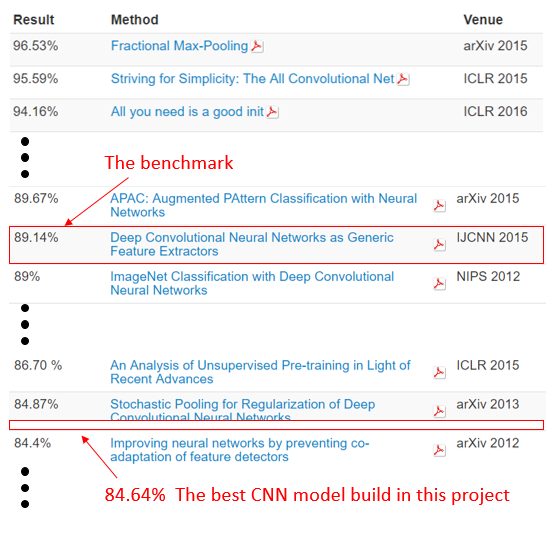
\includegraphics[width=6cm]{Images/state_of_the_art_approaches.png}}
\caption{\label{fig:state_of_the_art_approaches} The state-of-the-art results.}
\end{figure}

Because the performance of the best CNN model build for CIFAR-10 dataset in this project is unstable, in future, we want to solve this problem first. Another interesting direction that we come up with is that making computer automatically built neural networks for different dataset. Since the design of the architecture of deep neural networks is an extremely time consuming task, and most of the parameter tuning work we did in this project is programmable, we believe it is meaningful to make this process automatic.
%\begin{figure}[h]
%\centering
%\fboxsep 2mm
%\framebox{
%	
\includegraphics[width=6cm]{UCD_Logo} 
%	
\includegraphics[width=3cm]{UCD_Logo} 
%	\includegraphics[width=1.5cm]{UCD_Logo} 
%	\includegraphics[width=0.75cm]{UCD_Logo} 
%	\includegraphics[width=0.375cm]{UCD_Logo}
%}
%\caption{\label{fig:logo} Logo of the UCD Department of Computer Science displayed at various size.}
%\end{figure} 

%If you wish to print a short excerpt of your source code,  ensure that you are using a fixed-width sans-serif font such as the Courier font. Your code will be properly indented and will appear as follows:

%\begin{verbatim}
%let names = ["Science", "Computer", "of", "School", "UCD"]
%func backwards(s1: String, s2: String) -> Bool
%{
%   return s1 > s2
%}
%var reversed = sorted(names, backwards)
%// reversed is equal to ["UCD", "School", "of", "Computer", "Science"]
%\end{verbatim}


%%%% ADD YOUR BIBLIOGRAPHY HERE
\newpage
\bibliography{Reference} 
\bibliographystyle{ieeetr}

%\begin{thebibliography}{99}
%\bibitem{Gibson:2017} Gibson, A., \& Patterson, J. (2017). Deep Learning. Sebastopol: O’Reilly Media.
%\bibitem{Bonnin:2016} Bonnin, R. (2016). Building Machine Learning Projects with TensorFlow. Birmingham: Pack Publishing Ltd.
%\bibitem{Goodfellow:2000} Goodfellow, I., Bengio, Y., \& Courville, A. (2016). Deep Learning. Massachusetts: The MIT Press.
%\bibitem{Zhou:2016} Zhou, Z.H. (2016). Machine Learning. Beijing: Tsinghua University Press.
%\bibitem{Lars:2015} Lars H 
%\end{thebibliography}

\label{endpage}
\end{document}

\end{article}
